\documentclass{article}
\usepackage{geometry}
 \geometry{
 a4paper,
 total={170mm,257mm},
 left=20mm,
 top=20mm,
 }
 
 \usepackage{amsmath}
 \usepackage{diagbox}
 \usepackage{booktabs}
\usepackage{colortbl}

 \usepackage{caption}
\usepackage[export]{adjustbox} %% for picture frame
\usepackage[english]{babel}
\usepackage[utf8]{inputenc}
\usepackage{fancyhdr}

%%%question enviroment 

%%% Question Environment%%%  use 
%%% Question Environment%%%  use 
%%% Question Environment%%%  use \input{./QueENV.tex}   to include
%% Use \begin{Q}....\end{Q}

\newcounter{QC}
\setcounter{QC}{1}
\newenvironment{Q}[1]{
    \section{Question -\arabic{QC}} \stepcounter{QC}{\large\textbf{#1}}
}

%%% Question Environment%%%

   to include
%% Use \begin{Q}....\end{Q}

\newcounter{QC}
\setcounter{QC}{1}
\newenvironment{Q}[1]{
    \section{Question -\arabic{QC}} \stepcounter{QC}{\large\textbf{#1}}
}

%%% Question Environment%%%

   to include
%% Use \begin{Q}....\end{Q}

\newcounter{QC}
\setcounter{QC}{1}
\newenvironment{Q}[1]{
    \section{Question -\arabic{QC}} \stepcounter{QC}{\large\textbf{#1}}
}

%%% Question Environment%%%



\pagestyle{fancy}
\fancyhf{}
\rhead{\textit{LAB-4}}
\lhead{\textit{Pul074BEX004}}
\rfoot{\thepage}

%%% format and command for lab ans vhdl

%%% Formating And Command for Embedded Lab  VHDl
%% \ancode{caption}{Filename}


\usepackage{listings}
\usepackage{multicol}
\usepackage{mdframed}

\renewcommand{\lstlistlistingname}{List of VHDLCodes}
\renewcommand{\lstlistingname}{Code}

\setlength{\columnsep}{0.5cm}

\usepackage{xcolor}
\definecolor{codegreen}{rgb}{0,0.6,0}
\definecolor{codegray}{rgb}{0.4,0.4,0.4}
\definecolor{codepurple}{rgb}{0.58,0,0.82}
%\definecolor{backcolour}{rgb}{0.95,0.99,0.92}
\definecolor{backcolour}{rgb}{0,0,0}

\lstdefinestyle{VHDL}{
  backgroundcolor=\color{backcolour},   commentstyle=\color{codegreen},
  keywordstyle=\color{cyan},
  numberstyle=\tiny\color{codegray},
  stringstyle=\color{codepurple},
  basicstyle=\ttfamily\footnotesize\color{white},
  breakatwhitespace=false,
  breaklines=true,
  captionpos=b,
  morekeywords={LIBRARY, USE ,ALL,ENTITY,IS,PORT,IN,OUT,END,ARCHITECTURE, CONFIGURATION, OF, BODY,FUNCTION, VARIABLE, BEGIN,AND,OR,NOT, XOR, DOWNTO,ALL, SIGNAL, PROCESS, IF,
      ELSE, ELSIF, CASE, WHEN, THEN, RANGE, TO, COMPONENT, TYPE, WITH, SELECT,
      OTHERS, CONSTANT, INOUT, BUFFER, MAP, TRUE, FALSE, ARRAY, SUBTYPE, WAIT,
      WAIT FOR, GENERIC, =, <, >, <=, >=, =>},
  keepspaces=true,
  language=VHDL,
  numbers=left,
  numbersep=5pt,
  showspaces=false,
  showstringspaces=false,
  showtabs=false,
  tabsize=3
}




\newcommand {\anscode}[2]{

  \begin{center}
    \textbf{ $
        \Downarrow $ #2  $\Downarrow  $ }
  \end{center}
  \begin{multicols}{2}
    \lstinputlisting[style=VHDL,nolol]{#2}
  \end{multicols}

  \begingroup
  \captionof{lstlisting}{#1}
  \endgroup

}

%%% Formating And Command for Embedded Lab  VHDL
%%%%>>>>>>>........
%%%%%% include  Titles.%%%% use \input{./CP}%%%
%%%use """"""""    \CP{}{}{}{}   """" %%%% and 4 argument to craete Title page 
%%%%%%%%%%%%%%%%%%%%%%%%%%%%%%%%%%%%%%%%%%%%%%%%%%%%%%%%%%%%%%%%%
%%%argument number
%% 1=major header ## Course name 
%% 2=minor4 heading ## lab/assignmet no
%% 3=Title  ## Assignment or Lab title
%% 4=submitted to::## input receiver Name"
%%%%%%%%%%%%%%%%%%%%%%%%%%%%%%%%%%%%%%%%%%%%%%%%%%%%%%%%%%%%%%%%%


\usepackage{mathpazo} % Palatino font
\usepackage{graphicx}
\usepackage{float}

%%% format and command for lab ans c and assembly

\newcommand{\HRule}{\rule{\linewidth}{0.4mm}} % Defines a new command for horizontal lines, change thickness here



%----------------------------------------------------------------------------------------
%	TITLE PAGE
%----------------------------------------------------------------------------------------


\newcommand{\CP}[4]{ \begin{titlepage} % Suppresses displaying the page number on the title page and the subsequent page counts as page 1
		%%%%  univerdity logo%%
		\begin{figure}[H]
			\centering
			
\includegraphics[scale=0.13]{tulogo.jpg}
		\end{figure}
		%%% end university logo

		\center % Centre everything on the page

		%------------------------------------------------
		%	Headings
		%------------------------------------------------

		\textsc{\huge Institute of Engineering \\ Central Campus,Pulchowk}\\[1.5cm] % Main heading such as the name of your university/college

		\textsc{\Large #1}\\[0.5cm] % Major heading such as course name

		\textsc{\large #2}\\[0.5cm] % Minor heading such as assignment no./ lab no.

		%------------------------------------------------
		%	Title
		%------------------------------------------------

		\HRule\\[0.4cm]

		{\Huge\bfseries #3}\\[0.4cm] % Title of your document

		\HRule\\[1.5cm]

		%------------------------------------------------
		%	Author(s)
		%------------------------------------------------
		\vfill\vfill
		\begin{minipage}{0.4\textwidth}
			\begin{flushleft}
				\large{
				\textbf{Submitted BY:}\\
				{\normalsize AMRIT PRASAD PHUYAL}\\ % NAME
				{\normalsize Roll: PULL074BEX004}} % Roll
			\end{flushleft}
		\end{minipage}
		~
		\begin{minipage}{0.4\textwidth}
			\begin{flushright}
				\large
				\textbf{Submitted To:}\\
				{ \normalsize{#4}\\ }% recepent's  Name 
				{\normalsize Department of Electronics and Computer Engineering}
			\end{flushright}
		\end{minipage}

		%------------------------------------------------
		%	Date
		%------------------------------------------------

		\vfill\vfill\vfill % Position the date 3/4 down the remaining page

		{\large\today} % Date, change the \today to a set date if you want to be precise

		\vfill % Push the date up 1/4 of the remaining page

	\end{titlepage}
}


%%%for sub figures
%% File names should be adder-1, adder-2, and so on for adder and subtractor-1, subtractor-2, and so on for subtractor
%% use as \figures{adder} or \figures{substractor}
\usepackage{float}
\usepackage{pgffor}

\usepackage{caption}
\usepackage{subcaption}

\newcommand{\figures}[1]{
    \begin{figure}[H]
        \centering
        \foreach \i in {1,2,3}
            {
                \begin{subfigure}{\linewidth}
                    \includegraphics[width=.95\linewidth, frame]{../Figures/#1-\i.pdf}
                    \caption{}
                    \label{fig:obs7-\i}
                \end{subfigure}
            }
        \caption{Observed waveform for Problem 7}
        \label{fig:obs7}
    \end{figure}
    \begin{figure}[H]\ContinuedFloat
        \centering
        \foreach \i in {4,5,6}
            {
                \begin{subfigure}{\linewidth}
                    \includegraphics[width=.95\linewidth, frame]{../Figures/#1-\i.pdf}
                    \caption{}
                    \label{fig:obs7-\i}
                \end{subfigure}
            }
        \caption*{Figure~\ref{fig:obs7}:~Observed waveform for Problem 7- #1 (continued)}
    \end{figure}
    \begin{figure}[H]\ContinuedFloat
        \centering
        \foreach \i in {7,8,9}
            {
                \begin{subfigure}{\linewidth}
                    \includegraphics[width=.95\linewidth, frame]{../Figures/#1-\i.pdf}
                    \caption{}
                    \label{fig:obs7-\i}
                \end{subfigure}
            }
        \caption*{Figure~\ref{fig:obs7}:~Observed waveform for Problem 7- #1 (continued)}
    \end{figure}
    \begin{figure}[H]\ContinuedFloat
        \centering
        \foreach \i in {10,11,12}
            {
                \begin{subfigure}{\linewidth}
                    \includegraphics[width=.95\linewidth, frame]{../Figures/#1-\i.pdf}
                    \caption{}
                    \label{fig:obs7-\i}
                \end{subfigure}
            }
        \caption*{Figure~\ref{fig:obs7}:~Observed waveform for Problem 7- #1 (continued)}
    \end{figure}
    \begin{figure}[H]\ContinuedFloat
        \centering
        \foreach \i in {13,14,15}
            {
                \begin{subfigure}{\linewidth}
                    \includegraphics[width=.95\linewidth, frame]{../Figures/#1-\i.pdf}
                    \caption{}
                    \label{fig:obs7-\i}
                \end{subfigure}
            }
        \caption*{Figure~\ref{fig:obs7}:~Observed waveform for Problem 7- #1 (continued)}
    \end{figure}
}


\begin{document}

%----------------------------------------------------------------------------------------
%	TITLE PAGE
%----------------------------------------------------------------------------------------
\CP{Embedded system}{LAB \#4}
{Combinational Logic Design Using VHDL}
{Department of Electronics and Computer Engineering}




%----------------------------------------------------------------------------------------
\pagenumbering{gobble}
\tableofcontents
\pagebreak
\listoffigures
\pagebreak
\lstlistoflistings
\pagebreak
\pagenumbering{arabic}


\section{Title} {\large Combinational Logic Design Using VHDL}
%%%%%%%%%%%%%%%%%%%%%%%%%%%%
\section{Objective}
To enable us to write VHDL code for a Field Programmable Gate Array (FPGA) capableof:
\begin{itemize}
    \item Implementing combinational circuits
    \item Implementing test benches to verify the working of combinational circuits

\end{itemize}
%%%%%%%%%%%%%%%%%%%%%
\section{Requirement}

\textbf{Hardware:}

\begin{itemize}
    \item Spartan-3E or Spartan-3AN FPGA starter kit
    \item Power cable and Data cableSoftware:
\end{itemize}


\textbf{Software:}

\begin{itemize}
    \item Xilinx ISE (Integrated Synthesis Environment) Design Suite
    \item iMPACT configuration tool
\end{itemize}

\section{Introduction}
VHDL stands  for  Very  High  Speed  Integrated  Circuit  (VHSIC)  Hardware  DescriptiveLanguage. It is one of the programming languages which is used to model the digital circuits by  using  different  style  of modelling such  as  dataflow,  behavioral  and  structural.It  is  an event driven language, it means whenever an event occurs on signals in VHDL,it triggers the execution of a statement. It allows both concurrent as well as sequential modelling. It is case-insensitive  and  is  a  strongly  typed  language,  that  is,  it  does not support  implicit  conversion between  data  types.  It  supports  code  reusability  and  code sharing  via  packages  and  user defined libraries.In VHDL, an entity is used to describe a hardware module. An entity can be described using,

\begin{itemize}
    \item Entity declaration
    \item Architecture
    \item Configuration
    \item Package Declaration
    \item Package Body
\end{itemize}


\subsubsection{Features of VHDl}
\begin{itemize}
    \item It is a hardware descriptive language used for design
          entry and simulation of digital circuits.
    \item It is an event-driven language: i.e. whenever an event
          occurs on signals in VHDL, it triggers the execution of
          a statement.
    \item It allows both concurrent as well as sequential
          modelling.
    \item It gives the flexibility to define data types that are
          specific to user needs apart from predefined types.
    \item It supports code reusability and code sharing via
          packages and user defined libraries.
    \item It is case-insensitive i.e. it does not differentiate
          between lowercase and uppercase letters.
    \item It is strongly typed language i.e. it does not support
          implicit conversion between data types.
\end{itemize}


\pagebreak


\section{LAB Problems}
%%%%%%%%%%%%%%
%%%%%%%%%%%%%%
%%%%%%%%%%%%%%
%%%%%%%%%%%%%%
%%%%%%%%%%%%%%
%%%%%%%%%%%%%%
%%%%%%%%%%%%%%
%%%%%%%%%%%%%%%%%%%%%%%%%%%%%%%%%%%%%%%%%%%%1111111111111111111111111111111

% \addtocontents{lol}{\protect\subsection*{\HRule \\ Problem \\ \HRule}}
% \HRule
% \anscode{  }{}
% \HRule

%%%%%%%%%%%%%%
%%%%%%%%%%%%%%
%%%%%%%%%%%%%%
%%%%%%%%%%%%%%
%%%%%%%%%%%%%%
%%%%%%%%%%%%%%
%%%%%%%%%%%%%%
\begin{Q}
    {
        Write VHDL code to implement the logic circuit shown in below figure, which has4 inputs (x1, x2, x3 and x4) and one output (f).
        \begin{itemize}
            \item Provide the following architectural styles
                  \begin{enumerate}
                      \item Dataflow Style
                      \item  Behavioral Style
                      \item  Structural Style
                  \end{enumerate}
            \item Write a VHDL test bench to verify the operation of the logic circuit.
            \item Provide a simulation waveform depicting all possible input cases.
        \end{itemize}
    }
\end{Q}

\addtocontents{lof}{\protect\subsection*{\HRule \\ Problem 1 \\ \HRule}}

\begin{figure}[H]
    \centering
    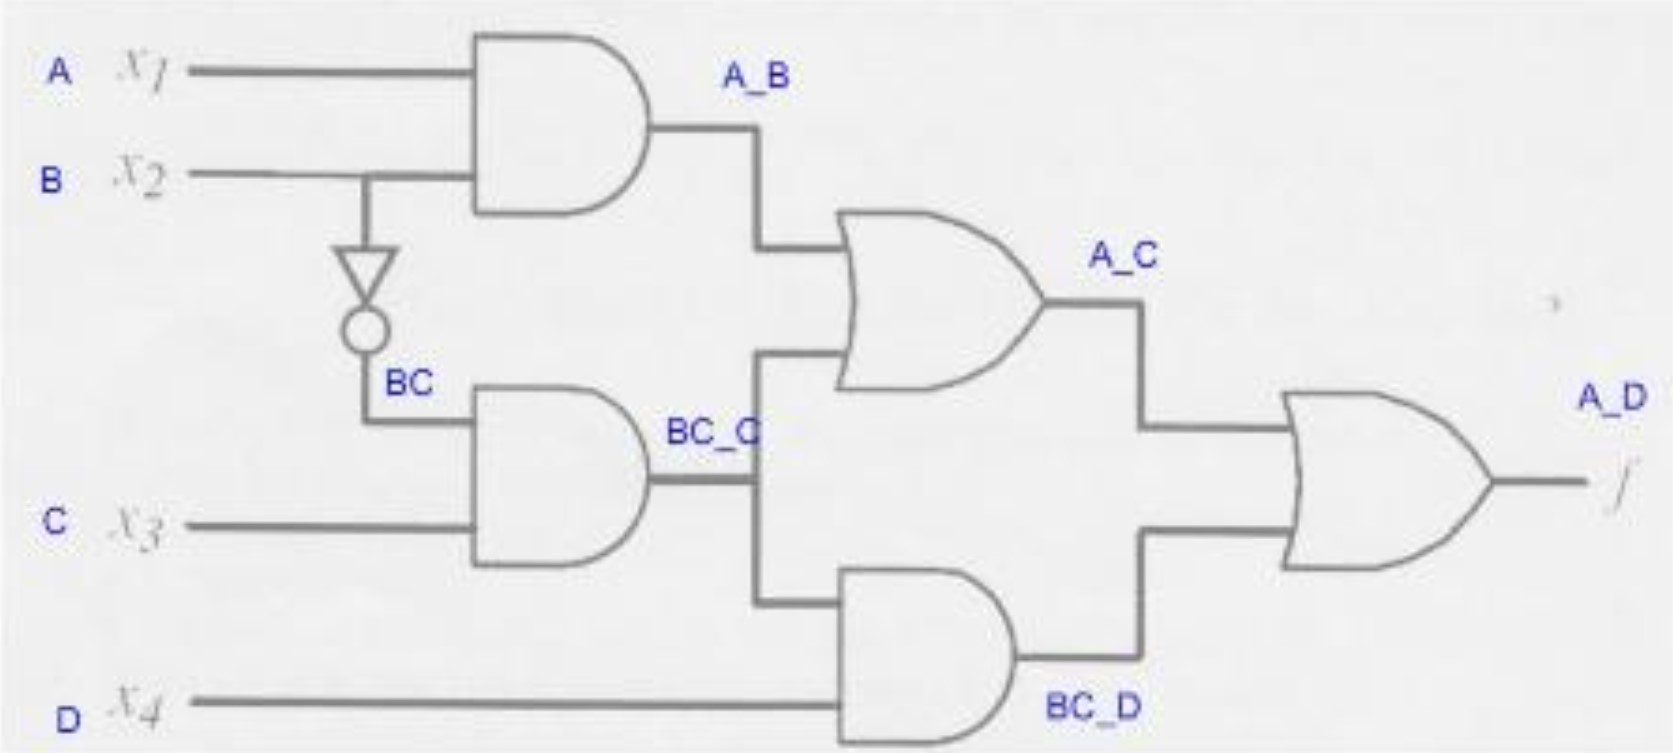
\includegraphics[scale=0.52,cframe=blue 0.5pt 3pt]{q1.jpg}
    \caption{Combinational Circuit for }
\end{figure}

\addtocontents{lol}{\protect\subsection*{\HRule \\ Problem 1 \\ \HRule}}

\HRule
\anscode{Dataflow model }{q1-df.vhd}
\HRule

\HRule
\anscode{AND gate  }{and1.vhd}
\HRule

\HRule
\anscode{OR gate }{or1.vhd}
\HRule

\HRule
\anscode{AND with one inverted variable}{andnot.vhd}
\HRule

\HRule
\anscode{Behavorial model }{q1-be.vhd}
\HRule

\HRule
\anscode{Structural model }{q1-st.vhd}
\HRule

\HRule
\anscode{Testbench for all cases }{q1-tb.vhd}
\HRule


%%%%%%%%%%%%waveform

\begin{figure}[H]
    \centering
    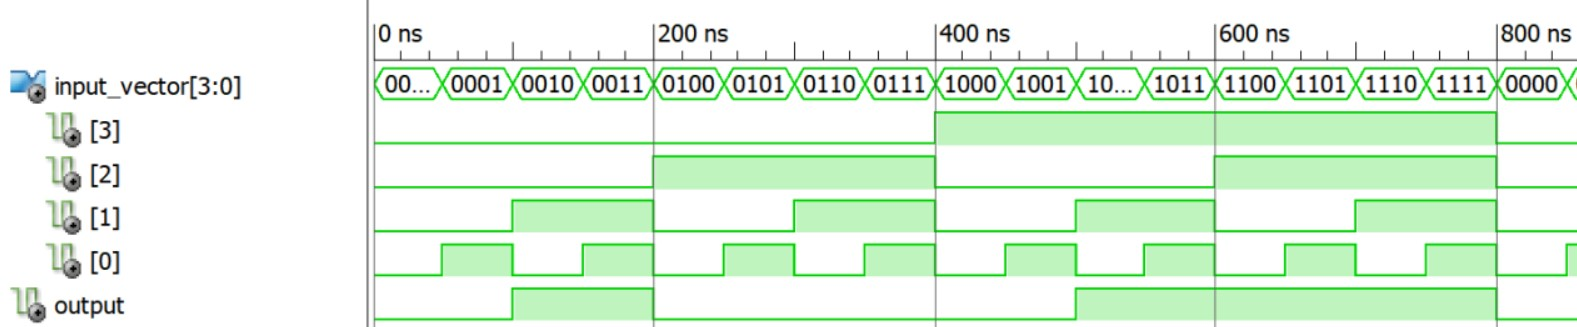
\includegraphics[scale=0.53,cframe=blue 0.5pt 3pt]{1w.jpg}
    \caption{Simulation Waveform }
\end{figure}


%%%RTL simulation
\begin{figure}[H]
    \centering
    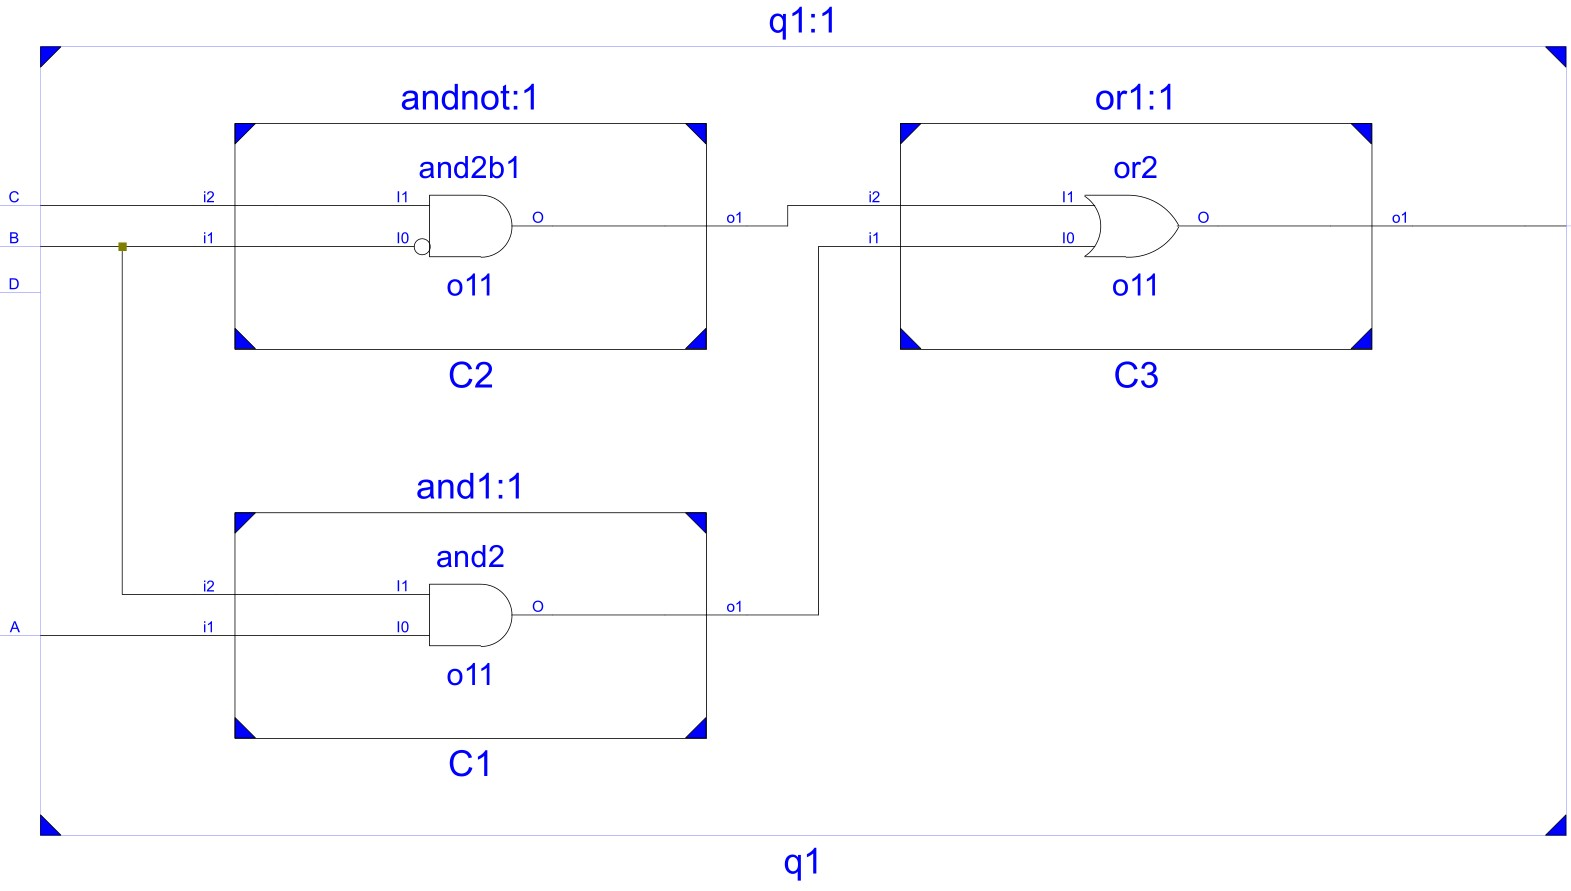
\includegraphics[scale=0.55,cframe=blue 0.5pt 3pt]{1s.jpg}
    \caption{RTL Schematic }
\end{figure}

%%%%%%%%%%%%%%
%%%%%%%%%%%%%%
%%%%%%%%%%%%%%
%%%%%%%%%%%%%%
%%%%%%%%%%%%%%
%%%%%%%%%%%%%%
%%%%%%%%%%%%%%

%%%%%%%%%%%%%%%%%%%%%%222222222222222222222222222222222
%%%%%%%%%%%%%%
%%%%%%%%%%%%%%
%%%%%%%%%%%%%%
%%%%%%%%%%%%%%
%%%%%%%%%%%%%%
%%%%%%%%%%%%%%
%%%%%%%%%%%%%%

\begin{Q}
    {
        Write VHDL code to design a logic circuit that implements the truth table of BCD-to-Gray
        code converter.
        \begin{enumerate}
            \item Use Karnaugh maps to simplify the output function.
            \item   Provide the following architectural styles:
                  \begin{itemize}
                      \item Dateflow style
                      \item  Behavioral style
                      \item  Structural style using only NOR gates
                  \end{itemize}
            \item  Write a VHDL test bench to verify the operation of the logic circuit.
            \item Provide a simulation waveform depicting all possible input cases.
        \end{enumerate}
    }
\end{Q}

\addtocontents{lof}{\protect\subsection*{\HRule \\ Problem 2\\ \HRule}}

\HRule
\anscode{Dataflow model }{q2-df.vhd}
\HRule
\addtocontents{lol}{\protect\subsection*{\HRule \\ Problem 2\\ \HRule}}
\begin{figure}[H]
    \centering
    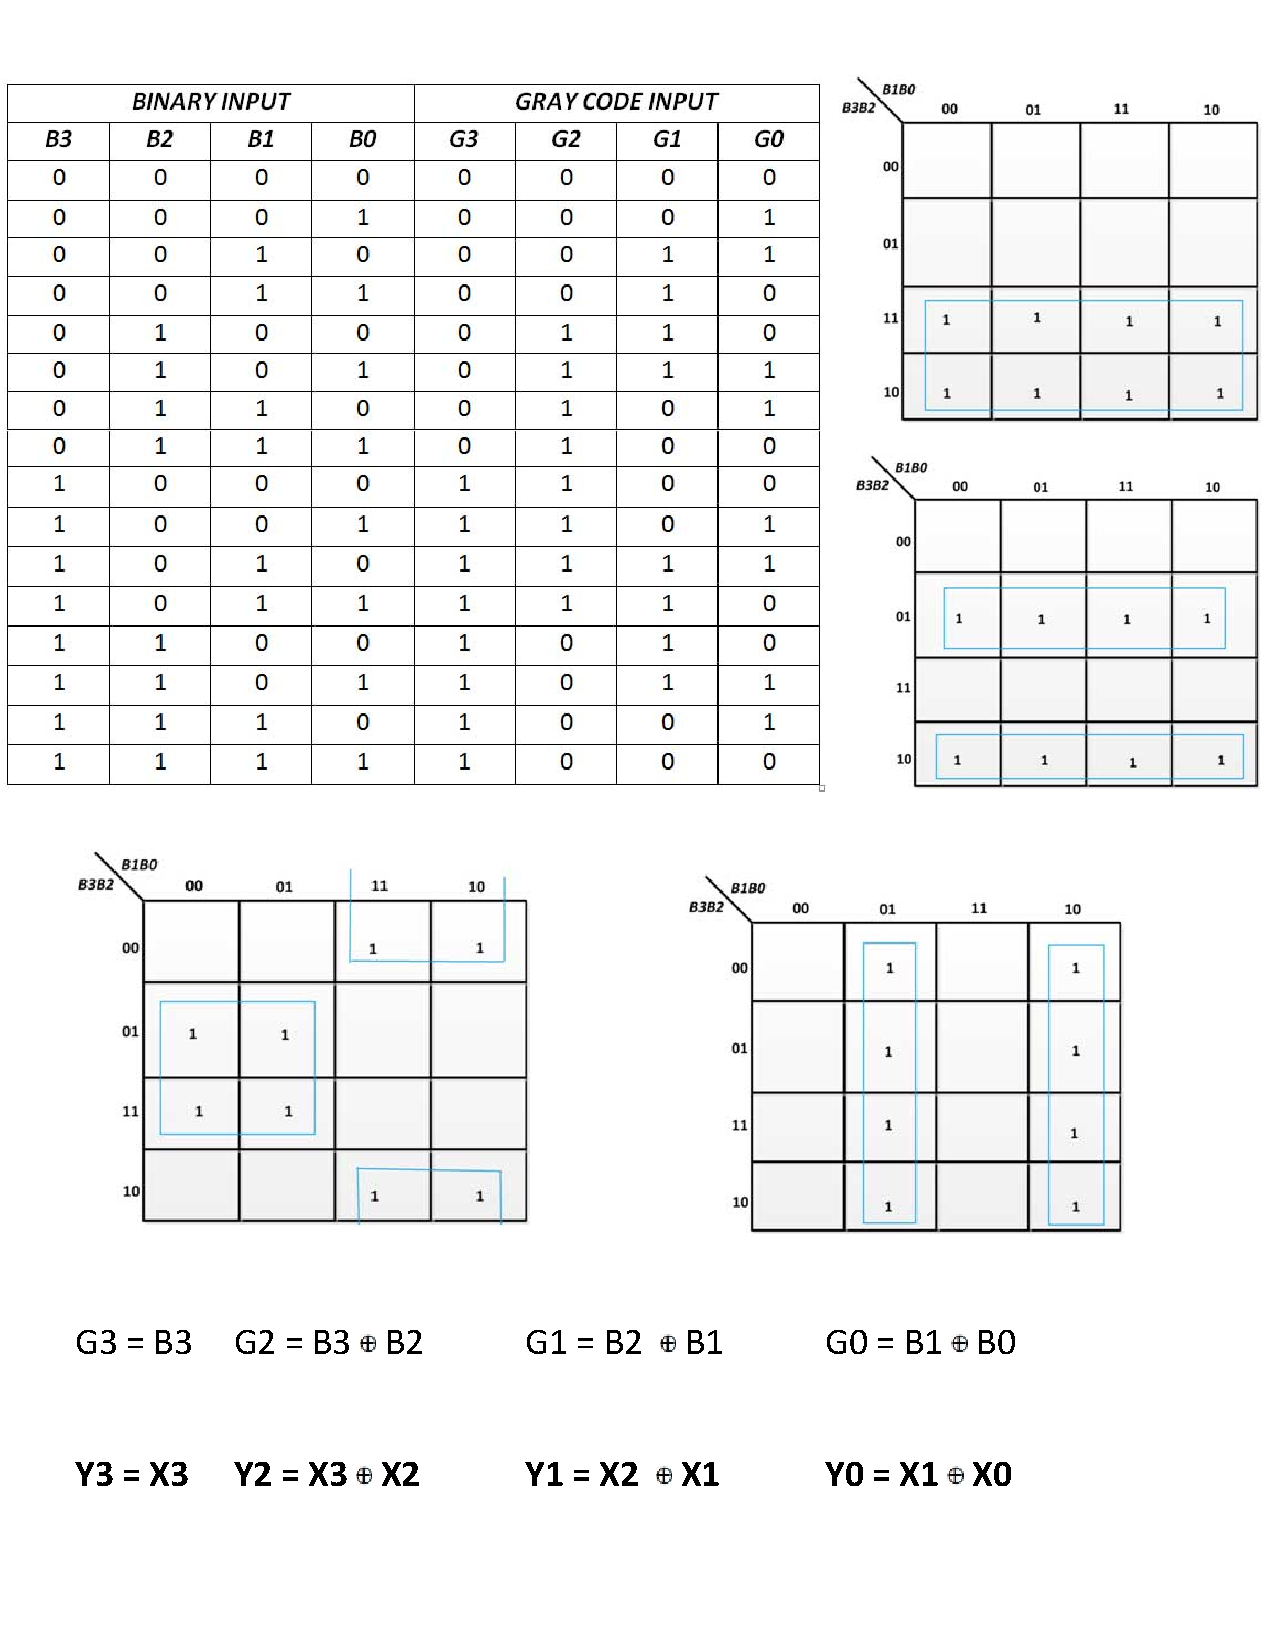
\includegraphics[scale=0.85,cframe=blue 0.5pt 3pt]{KMAP.pdf}
    \caption{BCD to Gray Code K map and Solution for }
\end{figure}

\anscode{Behavioral model }{q2-be.vhd}
\HRule

\HRule
\anscode{XOR gate }{xor-nor.vhd}
\HRule

\HRule
\anscode{Structural model }{q2-st.vhd}
\HRule

\HRule
\anscode{Testbench for all cases }{q2-tb.vhd}
\HRule

%%%%%%%%%%%%waveform

\begin{figure}[H]
    \centering
    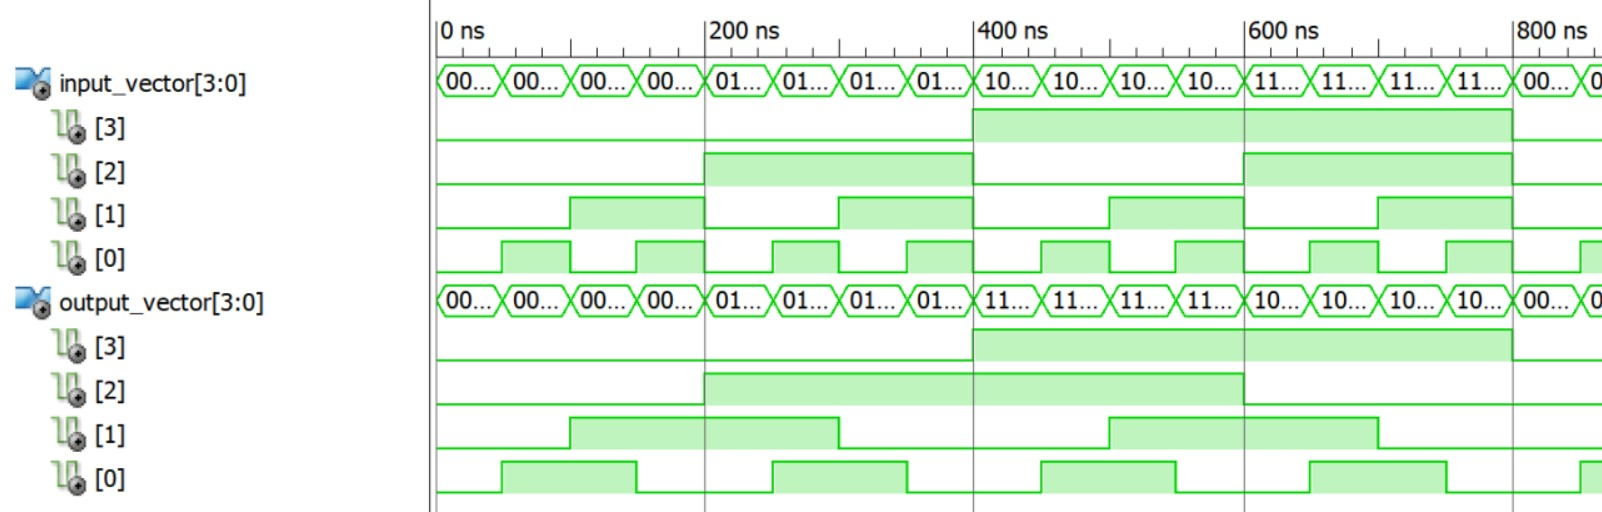
\includegraphics[scale=0.55,cframe=blue 0.5pt 3pt]{2w.jpg}
    \caption{Simulation Waveform }
\end{figure}


%%%RTL simulation
\begin{figure}[H]
    \centering
    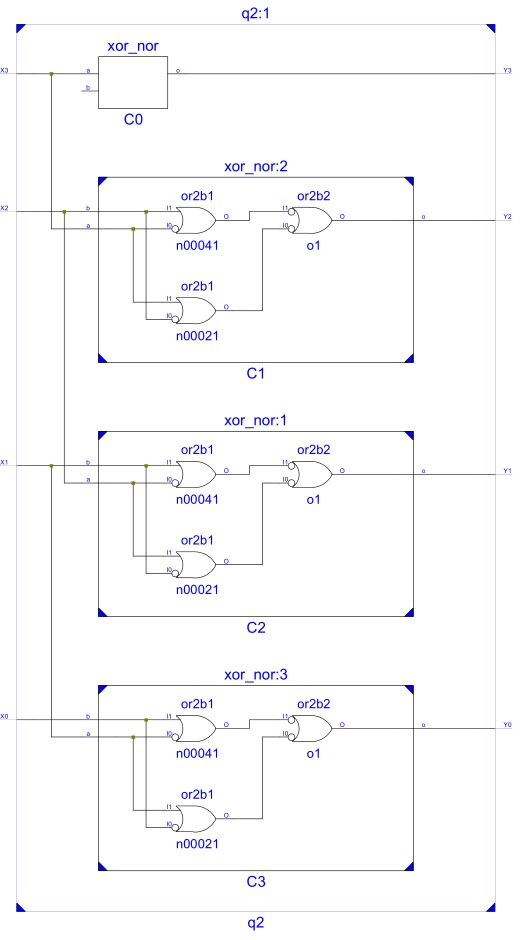
\includegraphics[scale=1.3,cframe=blue 0.5pt 3pt]{2s.jpg}
    \caption{RTL Schematic }
\end{figure}


%%%%%%%%%%%%%%
%%%%%%%%%%%%%%
%%%%%%%%%%%%%%
%%%%%%%%%%%%%%
%%%%%%%%%%%%%%
%%%%%%%%%%%%%%

%%%%%%%%%%%%%%%%%%%%%%33333333333333333333333333
%%%%%%%%%%%%%%
%%%%%%%%%%%%%%
%%%%%%%%%%%%%%
%%%%%%%%%%%%%%
%%%%%%%%%%%%%%
%%%%%%%%%%%%%%


\begin{Q}
    {
        Write VHDL code to implement the logic function (F) with the three input variables x1, x2,
        and x3. The function (F) is equal to 1 if and only if two variables are equal to 1; otherwise, it
        is equal to zero.
        \begin{enumerate}
            \item Draw a truth table for the function (F), and use Karnaugh maps to simplify
            \item   Provide the following architectural styles:
                  \begin{itemize}
                      \item Dateflow style
                      \item  Behavioral style
                      \item  Structural style using only NOR gates
                  \end{itemize}
            \item  Write a VHDL test bench to verify the operation of the logic circuit.
            \item Provide a simulation waveform depicting all possible input cases.
        \end{enumerate}
    }
\end{Q}
\addtocontents{lof}{\protect\subsection*{\HRule \\ Problem 3 \\ \HRule}}
% \usepackage{booktabs}
% \usepackage{colortbl}


\begin{table}[H]
    \centering
    \setlength{\extrarowheight}{0pt}
    \addtolength{\extrarowheight}{\aboverulesep}
    \addtolength{\extrarowheight}{\belowrulesep}
    \setlength{\aboverulesep}{0pt}
    \setlength{\belowrulesep}{0pt}

    \begin{tabular}{| m{5em}| m{5em}| m{5em}|m{5em}|}
        \toprule
        \rowcolor[rgb]{0.4,0.635,1} \multicolumn{3}{|l|}{Input} & Output                                 \\
        \hline
        \textbf{X3}                                             & \textbf{X2} & \textbf{X1} & \textbf{F} \\
        \hline
        0                                                       & 0           & 0           & 0          \\
        \hline
        0                                                       & 0           & 1           & 0          \\
        \hline
        0                                                       & 1           & 0           & 0          \\
        \hline
        0                                                       & 1           & 1           & 1          \\
        \hline
        1                                                       & 0           & 0           & 0          \\
        \hline
        1                                                       & 0           & 1           & 1          \\
        \hline
        1                                                       & 1           & 0           & 1          \\
        \hline
        1                                                       & 1           & 1           & 0          \\
        \bottomrule
    \end{tabular}
    \caption{Truth table Probelm 3}
\end{table}


% \usepackage{colortbl}
% \usepackage{booktabs}


\begin{table}[H]
    \centering
    \setlength{\extrarowheight}{0pt}
    \addtolength{\extrarowheight}{\aboverulesep}
    \addtolength{\extrarowheight}{\belowrulesep}
    \setlength{\aboverulesep}{0pt}
    \setlength{\belowrulesep}{0pt}

    \begin{tabular}{| m{8em}| m{5em}| m{5em}|m{5em}| m{5em}|}
        \toprule
        \diagbox{\textbf{X1}}{\textbf{X2 X1}} & \textbf{00} & \textbf{01}                 & \textbf{11}                            & \textbf{11}                   \\
        \hline
        \textbf{0}                            & 0           & 0                           & {\cellcolor[rgb]{0.027,1,1}}\textbf{1} & 0                             \\
        \hline
        \textbf{1}                            & 0           & {\cellcolor{red}}\textbf{1} & 0                                      & {\cellcolor{green}}\textbf{1} \\
        \bottomrule
    \end{tabular}
    \caption{K-map solution}
\end{table}


Expression Obtained is:
\begin{gather*}
    F=x_1x'_2x_3 + x'_1x_2x_3 + x_1x_2x'_3\\
    \quad \quad =((x'_1 + x_2 + x'_3)' (x_1 + x'_2 + x'_3)' (x'_1 + x'_2 + x_3'))
\end{gather*}

\addtocontents{lol}{\protect\subsection*{\HRule \\ Problem 3\\ \HRule}}
\HRule
\anscode{Dataflow model  }{q3-df.vhd}
\HRule

\HRule
\anscode{Behavorial model  }{q3-be.vhd}
\HRule

\HRule
\anscode{  NOT gate  using only NOR  }{q3-not.vhd}
\HRule

\HRule
\anscode{ 3-input OR gate  using only NOR }{q3-or.vhd}
\HRule

\HRule
\anscode{3-input AND gate  using only NOR  }{q3-and.vhd}
\HRule

\HRule
\anscode{  Structural model }{q3-st.vhd}
\HRule

\HRule
\anscode{  Testbench for all  cases}{q3-tb.vhd}
\HRule

%%%%%%%%%%%%waveform

\begin{figure}[H]
    \centering
    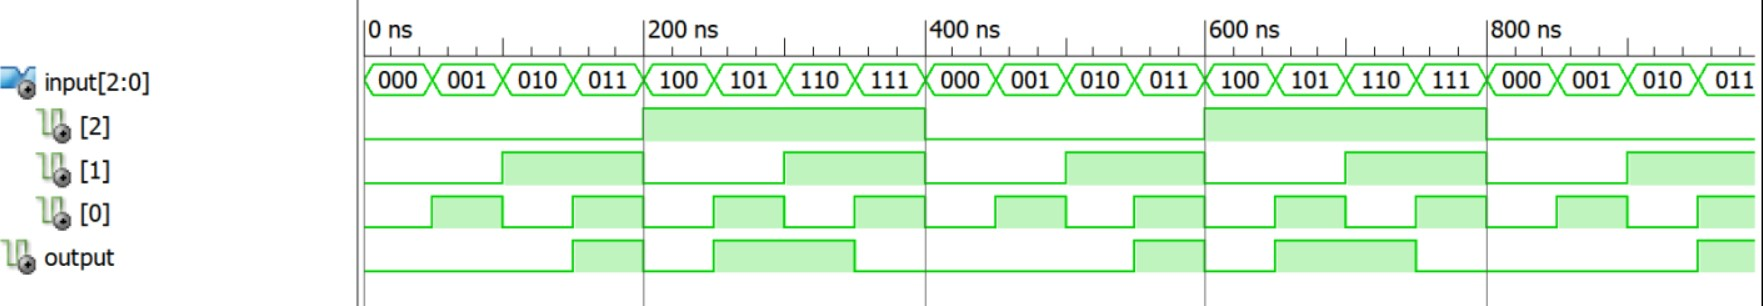
\includegraphics[scale=0.5,cframe=blue 0.5pt 3pt]{3w.jpg}
    \caption{Simulation Waveform for Problem 3}
\end{figure}


%%%RTL simulation
\begin{figure}[H]
    \centering
    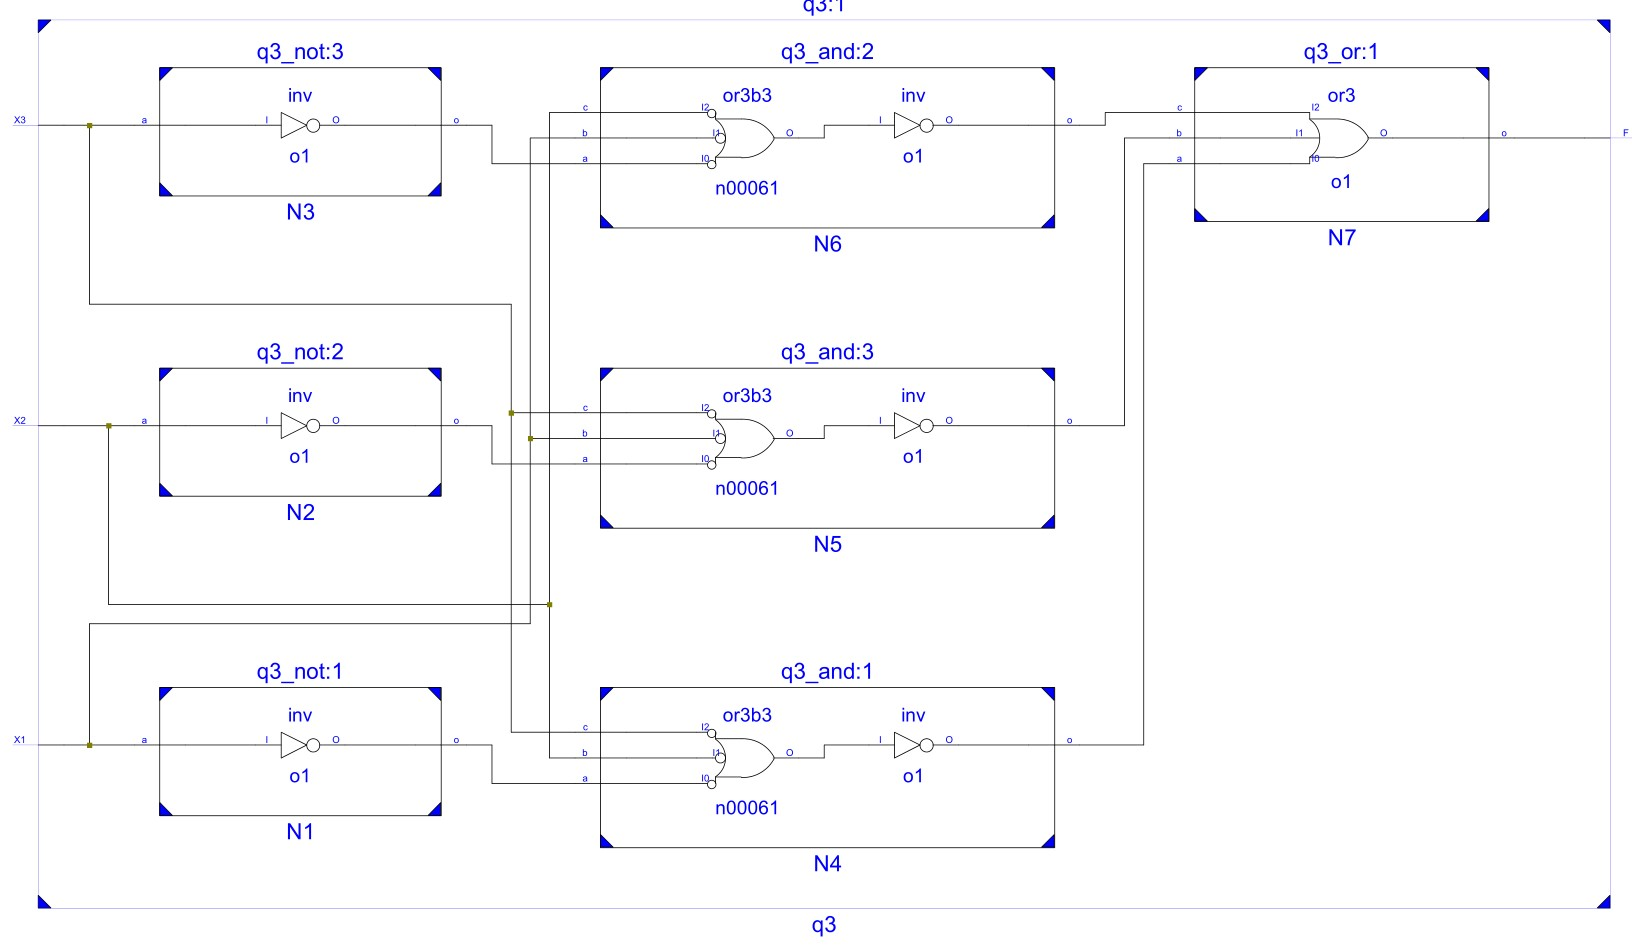
\includegraphics[scale=0.5,cframe=blue 0.5pt 3pt]{3s.jpg}
    \caption{RTL Schematic for Problem 3}
\end{figure}



%%%%%%%%%%%%%%
%%%%%%%%%%%%%%
%%%%%%%%%%%%%%
%%%%%%%%%%%%%%
%%%%%%%%%%%%%%
%%%%%%%%%%%%%%

%%%%%%%%%%%%%%%%%%%%%444444444444444444444444444444444
%%%%%%%%%%%%%%
%%%%%%%%%%%%%%
%%%%%%%%%%%%%%
%%%%%%%%%%%%%%
%%%%%%%%%%%%%%
%%%%%%%%%%%%%%
\begin{Q}
    {
        Write VHDL code to implement the implicit sum of products (SOP) and product of sums
        (POS) logic functions.
        \begin{align*}
            F(x_1,x_2,x_3,x_4)=\sum (m_0,m_1,m_4,m_5,m_8,m_9,m_{14},m_{15}) \\
            F(x_1,x_2,x_3,x_4)= \Pi (M_0,M_1,M_5,M_8,M_9,M_{13},M_{15})
        \end{align*}
        \begin{enumerate}
            \item Draw a truth table for the function (F), and use Karnaugh maps to simplify
            \item   Provide the following architectural styles:
                  \begin{itemize}
                      \item Dateflow style
                      \item  Behavioral style
                      \item  Structural style using only NOR gates
                  \end{itemize}
            \item  Write a VHDL test bench to verify the operation of the logic circuit.
            \item Provide a simulation waveform depicting all possible input cases.
        \end{enumerate}
    }
\end{Q}

\addtocontents{lof}{\protect\subsection*{\HRule \\ Problem 4 \\ \HRule}}

\begin{figure}[H]
    \centering
    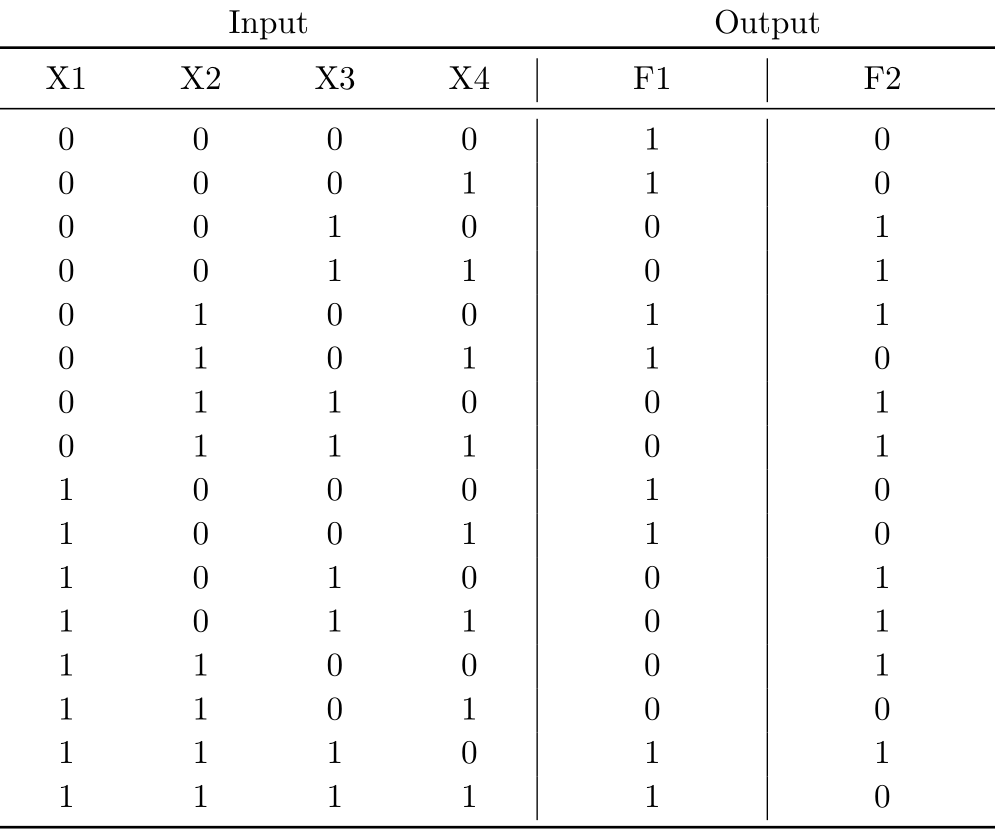
\includegraphics[scale=0.5,cframe=blue 0.5pt 3pt]{4TT.png}
    \caption{Truth table Problem 4}
\end{figure}



\begin{figure}[H]
    \centering
    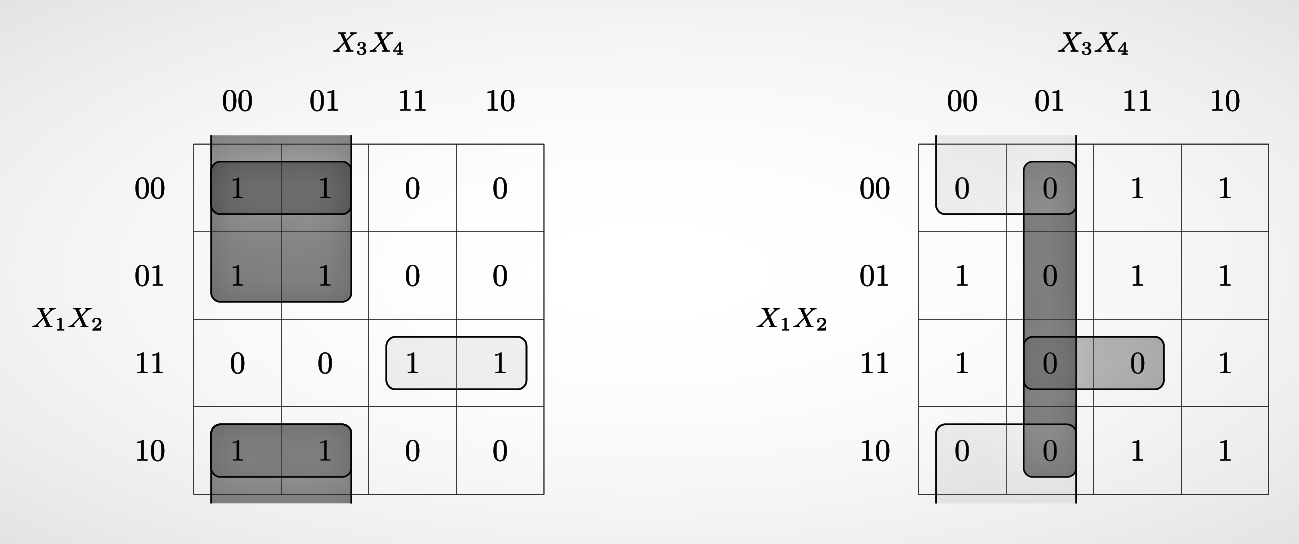
\includegraphics[scale=0.5,cframe=blue 0.5pt 3pt]{4km.png}
    \caption{SOP and POS K-map reduction F1 and F2}
\end{figure}




\begin{align*}
    F_1=X'_1X'_3 + X_1X_2X_3 + X'_2X'_3 \\
    F_2=(X_3 + X_4) (X'_1+ X'_2 + X'_4) (X_2 + X_3)
\end{align*}

\addtocontents{lol}{\protect\subsection*{\HRule \\ Problem 4\\ \HRule}}
\addtocontents{lol}{\protect\subsubsection*{ SOP }}
%%%%%%%%%%%%%%%%%%%%%%%SOP

\HRule
\anscode{  Dataflow model SOP }{q4sop-df.vhd}
\HRule

\HRule
\anscode{ Behavorial model SOP }{q4sop-be.vhd}
\HRule

\HRule
\anscode{ NOT gate implementation using only NOR }{q4-not.vhd}
\HRule

\HRule
\anscode{  3-input OR gate implementation using only NOR }{q4-or.vhd}
\HRule

\HRule
\anscode{  3-input AND gate implementation using only NOR }{q4-and.vhd}
\HRule

\HRule
\anscode{ Structural model  SOP}{q4sop-st.vhd}
\HRule

\HRule
\anscode{Testbench for all posible cases SOP }{q4sop-tb.vhd}
\HRule

%%%%%%%%%%%%waveform

\begin{figure}[H]
    \centering
    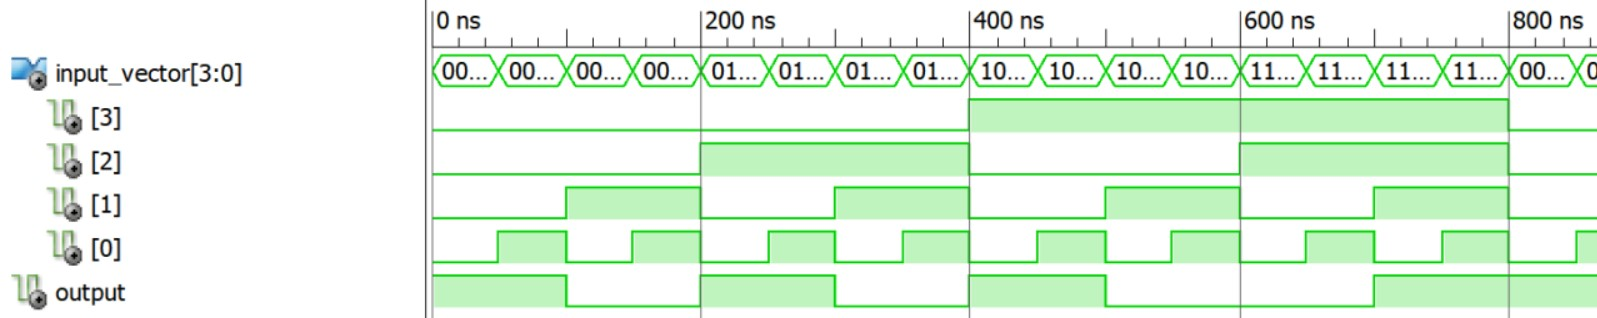
\includegraphics[scale=0.55,cframe=blue 0.5pt 3pt]{4sw.jpg}
    \caption{Simulation Waveform  SOP}
\end{figure}


%%%RTL simulation
\begin{figure}[H]
    \centering
    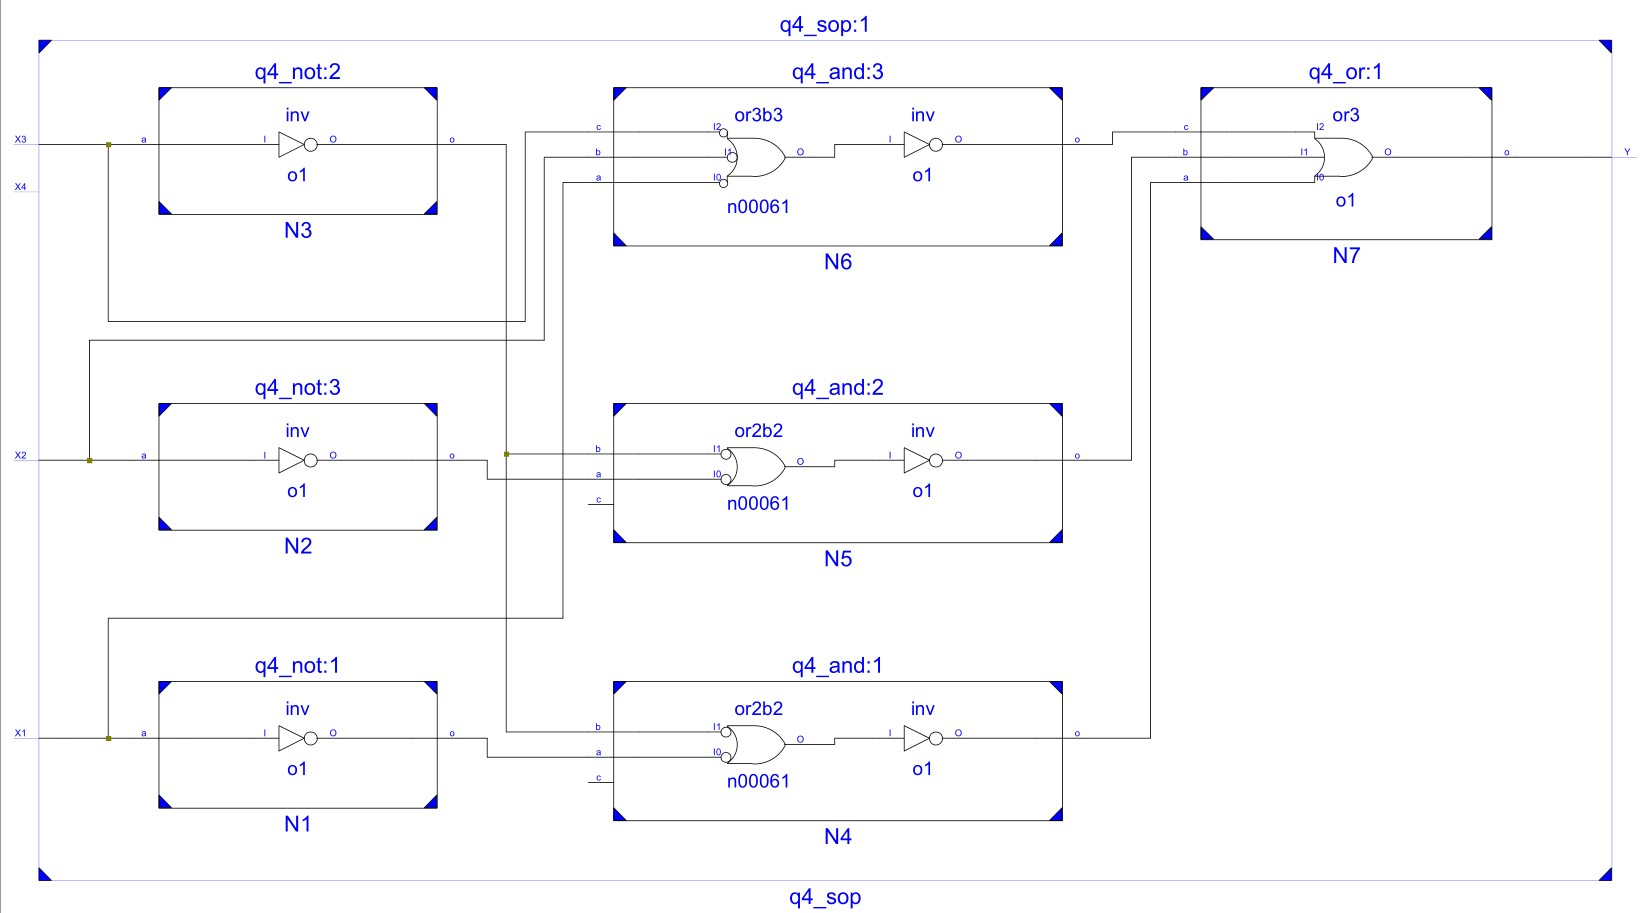
\includegraphics[scale=0.5,cframe=blue 0.5pt 3pt]{4ss.jpg}
    \caption{RTL Schematic  SOP}
\end{figure}


\addtocontents{lol}{\protect\subsubsection*{ POS }}

%%%%%%%%%%%%%%%%%%%%%%%%POS

\HRule
\anscode{  Dataflow model POS }{q4pos-df.vhd}
\HRule

\HRule
\anscode{ Behavorial model POS}{q4pos-be.vhd}
\HRule

\HRule
\anscode{ Structural model POS}{q4pos-st.vhd}
\HRule

\HRule
\anscode{ Testbench for all posible cases POS }{q4pos-tb.vhd}
\HRule

%%%%%%% waveform
\begin{figure}[H]
    \centering
    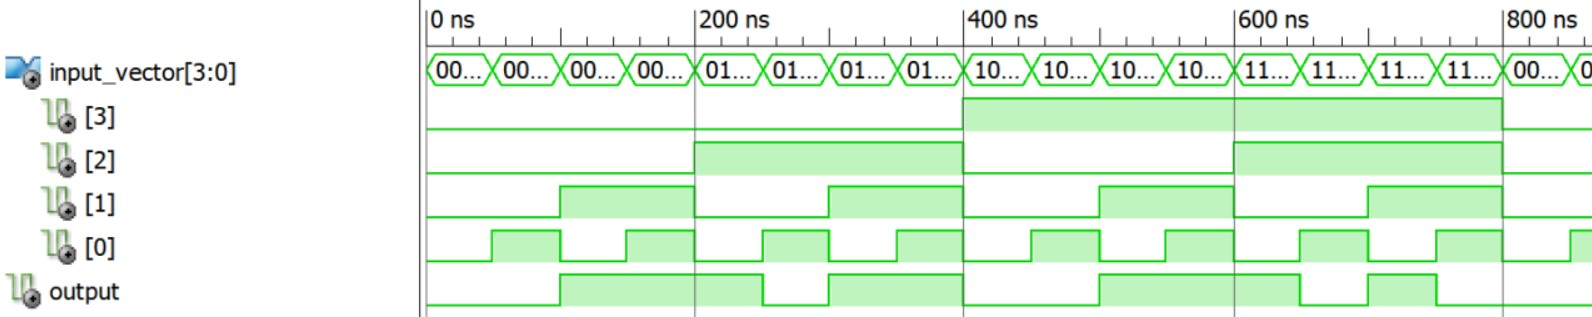
\includegraphics[scale=0.55,cframe=blue 0.5pt 3pt]{4pw.jpg}
    \caption{Simulation Waveform  POS}
\end{figure}


%%%RTL simulation
\begin{figure}[H]
    \centering
    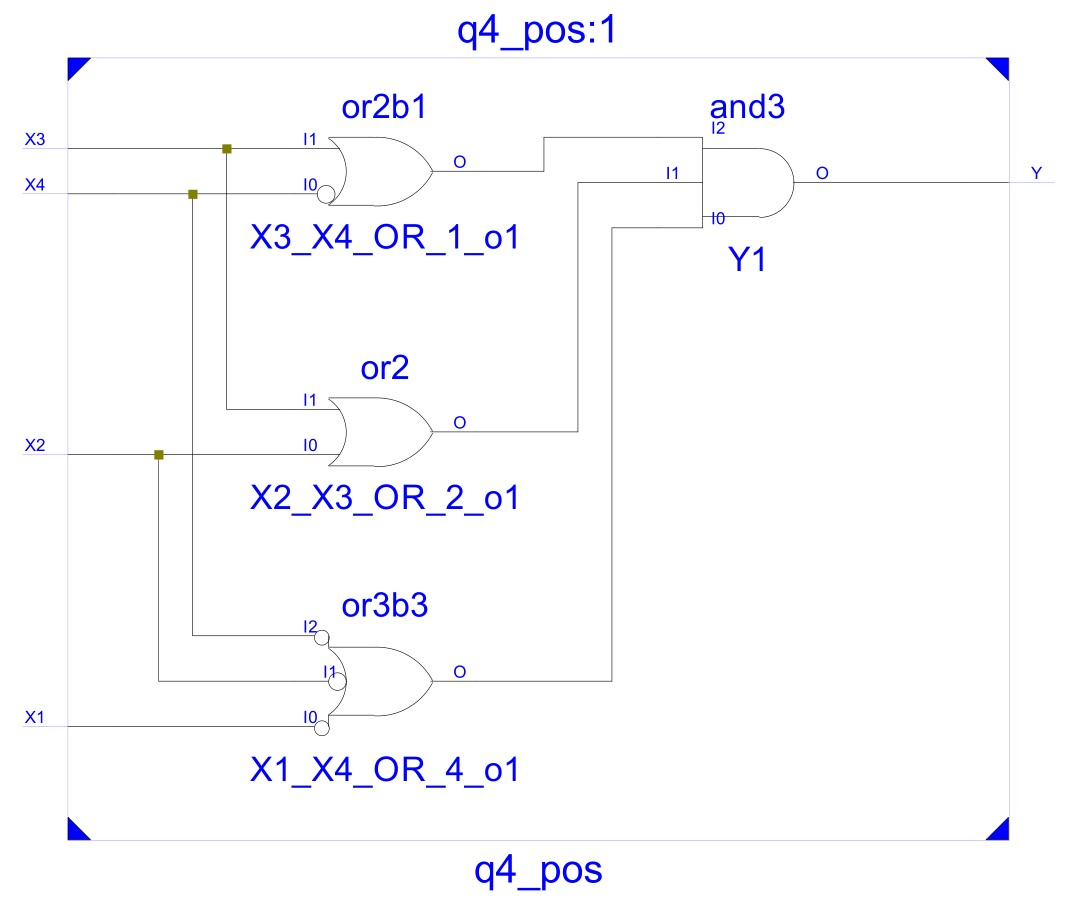
\includegraphics[scale=0.8,cframe=blue 0.5pt 3pt]{4ps.jpg}
    \caption{RTL Schematic  POS}
\end{figure}



%%%%%%%%%%%%%%
%%%%%%%%%%%%%%
%%%%%%%%%%%%%%
%%%%%%%%%%%%%%
%%%%%%%%%%%%%%
%%%%%%%%%%%%%%

%%%%%%%%%%%%%%%%%%%%%555555555555555555555555555555
%%%%%%%%%%%%%%
%%%%%%%%%%%%%%
%%%%%%%%%%%%%%
%%%%%%%%%%%%%%
%%%%%%%%%%%%%%

\begin{Q}
    {
        Write VHDL code to implement a 2:1 MUX having inputs x1 and x2, select line s and output
        y.
        \begin{enumerate}
            \item   Provide the following architectural implementations:
                  \begin{itemize}
                      \item Using WHEN-ELSE statement
                      \item IF-THEN-ELSE statement
                  \end{itemize}
            \item  Write a VHDL test bench to verify the operation of the  2:1 MUX.
            \item Provide a simulation waveform depicting all possible input cases.
        \end{enumerate}
    }
\end{Q}

\addtocontents{lof}{\protect\subsection*{\HRule \\ Problem 5 \\ \HRule}}
\addtocontents{lol}{\protect\subsection*{\HRule \\ Problem 5 \\ \HRule}}

\begin{figure}[H]
    \centering
    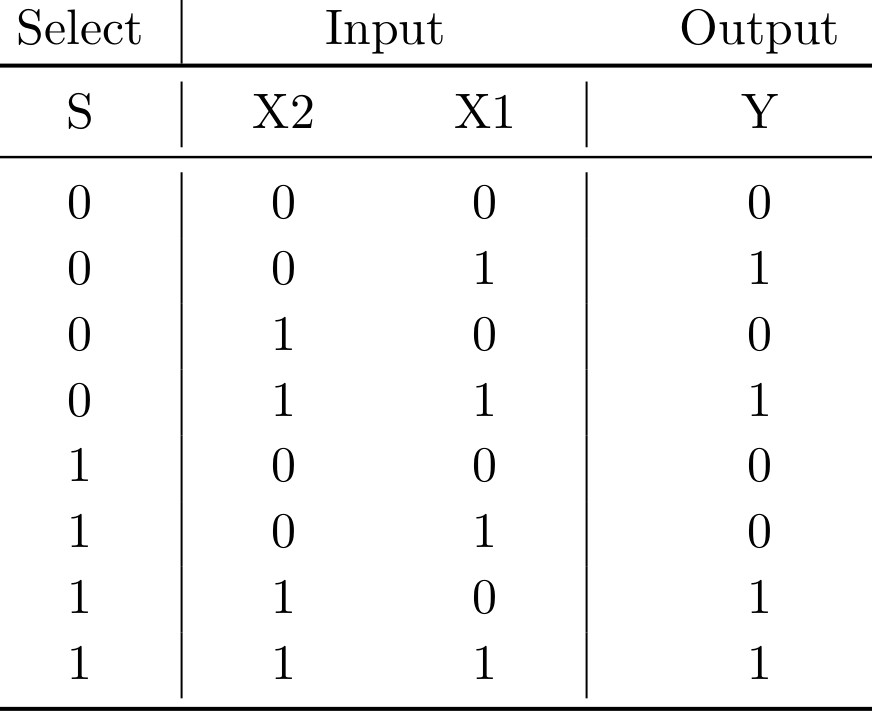
\includegraphics[scale=0.5,cframe=blue 0.5pt 3pt]{5tt.jpg}
    \caption{Truth Table 2:1 multiplexer}
\end{figure}

The required Boolean Equation is , $Y=SX_2 + S'X_1$

\HRule
\anscode{ 2:1 MUX implementation using WHEN-ELSE statement  }{q5-when-else.vhd}
\HRule

\HRule
\anscode{ 2:1 MUX implementation using IF-THEN-ELSE statement  }{q5-if-then-else.vhd}
\HRule


\HRule
\anscode{ Testbench for all possible cases  }{q5-tb.vhd}
\HRule



%%%%%%% waveform
\begin{figure}[H]
    \centering
    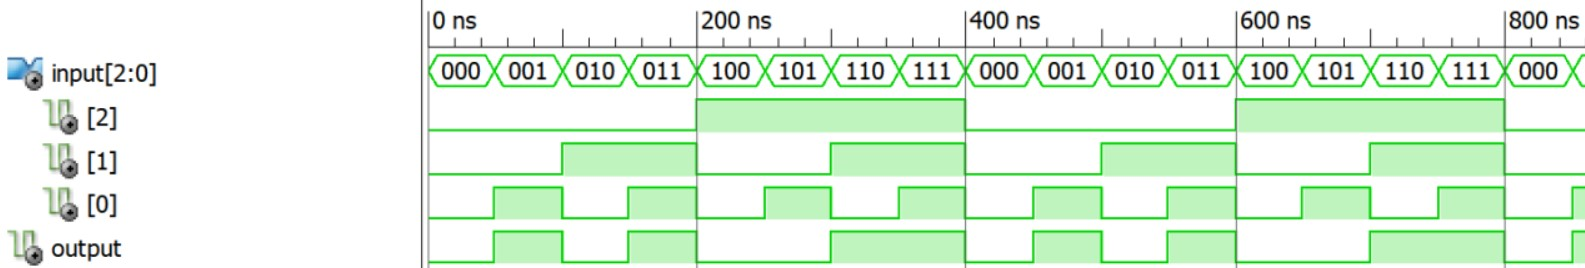
\includegraphics[scale=0.55,cframe=blue 0.5pt 3pt]{5w.jpg}
    \caption{Simulation Waveform  }
\end{figure}


%%%RTL simulation
\begin{figure}[H]
    \centering
    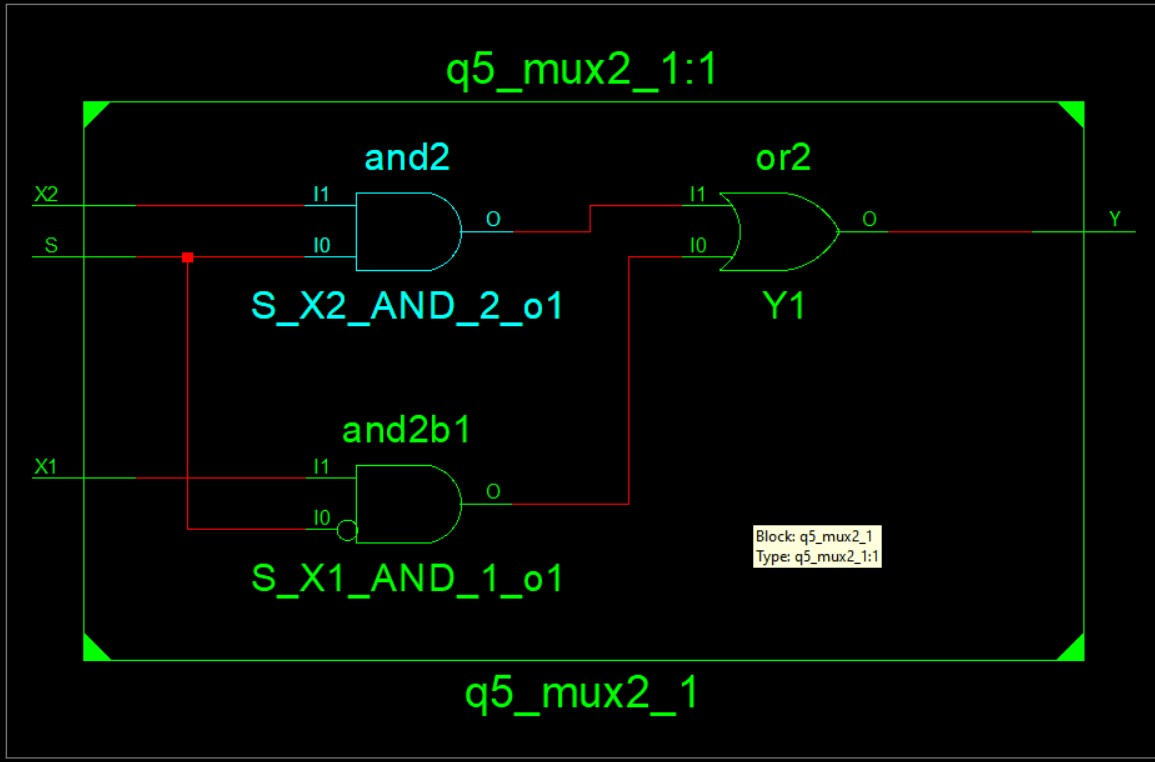
\includegraphics[scale=0.72,cframe=blue 0.5pt 3pt]{5s.jpg}
    \caption{RTL Schematic  }
\end{figure}




%%%%%%%%%%%%%%
%%%%%%%%%%%%%%
%%%%%%%%%%%%%%
%%%%%%%%%%%%%%
%%%%%%%%%%%%%%
%%%%%%%%%%%%%%

%%%%%%%%%%%%%%%%%%%%%6666666666666666666666666666666666666

%%%%%%%%%%%%%%
%%%%%%%%%%%%%%
%%%%%%%%%%%%%%
%%%%%%%%%%%%%%
%%%%%%%%%%%%%%

\begin{Q}
    {
        Write VHDL code to implement a 4:1 MUX having inputs x1, x2, x3 and x4, select lines s1,
        s0 and output y using three 2:1 multiplexers as the basic building blocks.
        \begin{enumerate}
            \item   Use a hierarchical design approach:
                  \begin{enumerate}
                      \item Create component definitions in separate (.vhd) files. Use either Dataflow or Behavioral or Structural
                            design styles.
                      \item Use Structural design style for the 4:1 MUX architecture:
                            \begin{enumerate}
                                \item Make use of 2:1 MUX component declaration.
                                \item Make use of 2:1 MUX component instantiation.
                            \end{enumerate}
                  \end{enumerate}
            \item  Write a VHDL test bench to verify the operation of the  2:1 MUX.
            \item Provide a simulation waveform depicting all possible input cases.
        \end{enumerate}
    }
\end{Q}

\addtocontents{lof}{\protect\subsection*{\HRule \\ Problem 6 \\ \HRule}}
\addtocontents{lol}{\protect\subsection*{\HRule \\ Problem 6 \\ \HRule}}

\begin{figure}[H]
    \centering
    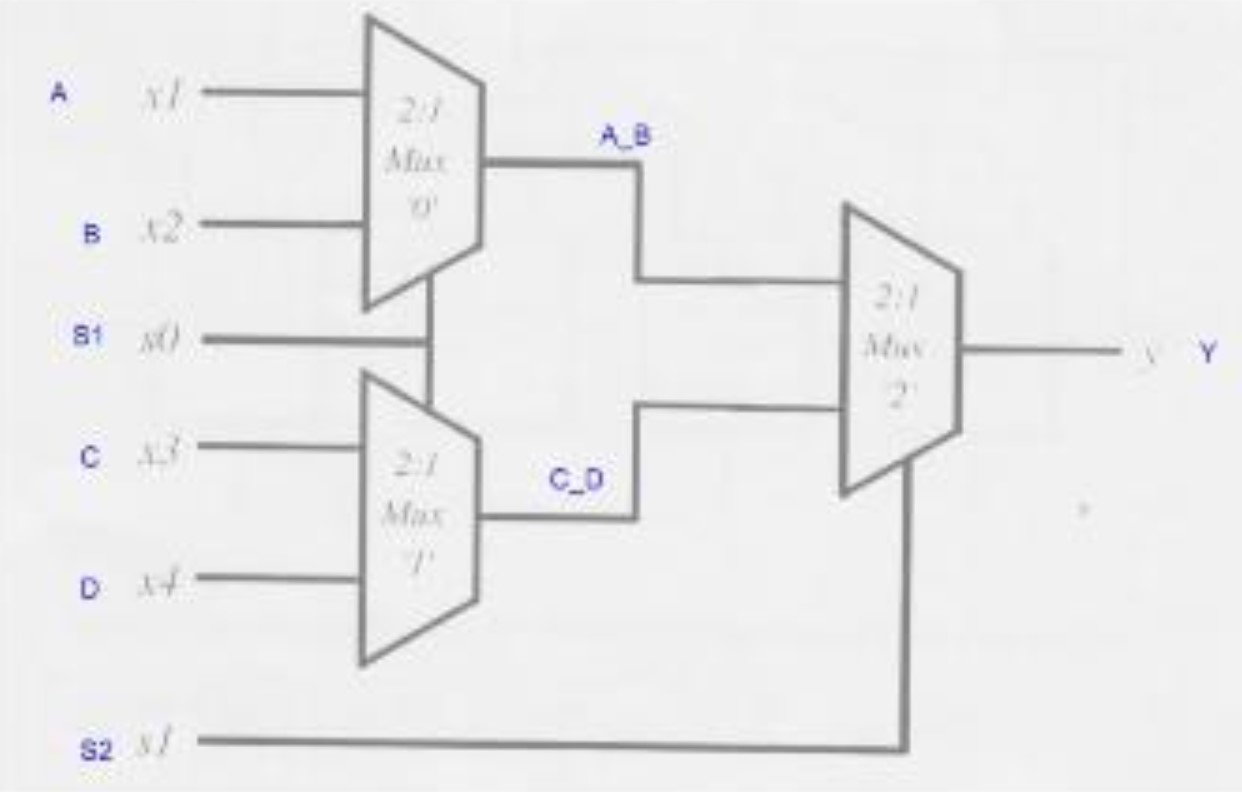
\includegraphics[scale=0.5,cframe=blue 0.5pt 3pt]{6.jpg}
    \caption{  MUX using three 2:1 MUX as basic building blocks }
\end{figure}


\HRule
\anscode{2:1 MUX implementation using WHEN-ELSE statement } {q5-when-else.vhd}
\HRule


\HRule
\anscode{ 4:1 MUX implementation using three 2:1 MUX: Structural model } {q6-st.vhd}
\HRule


\HRule
\anscode{Testbench for all possible cases} {q6-tb.vhd}
\HRule


%%%%%% waveform


\begin{figure}[H]
    \centering
    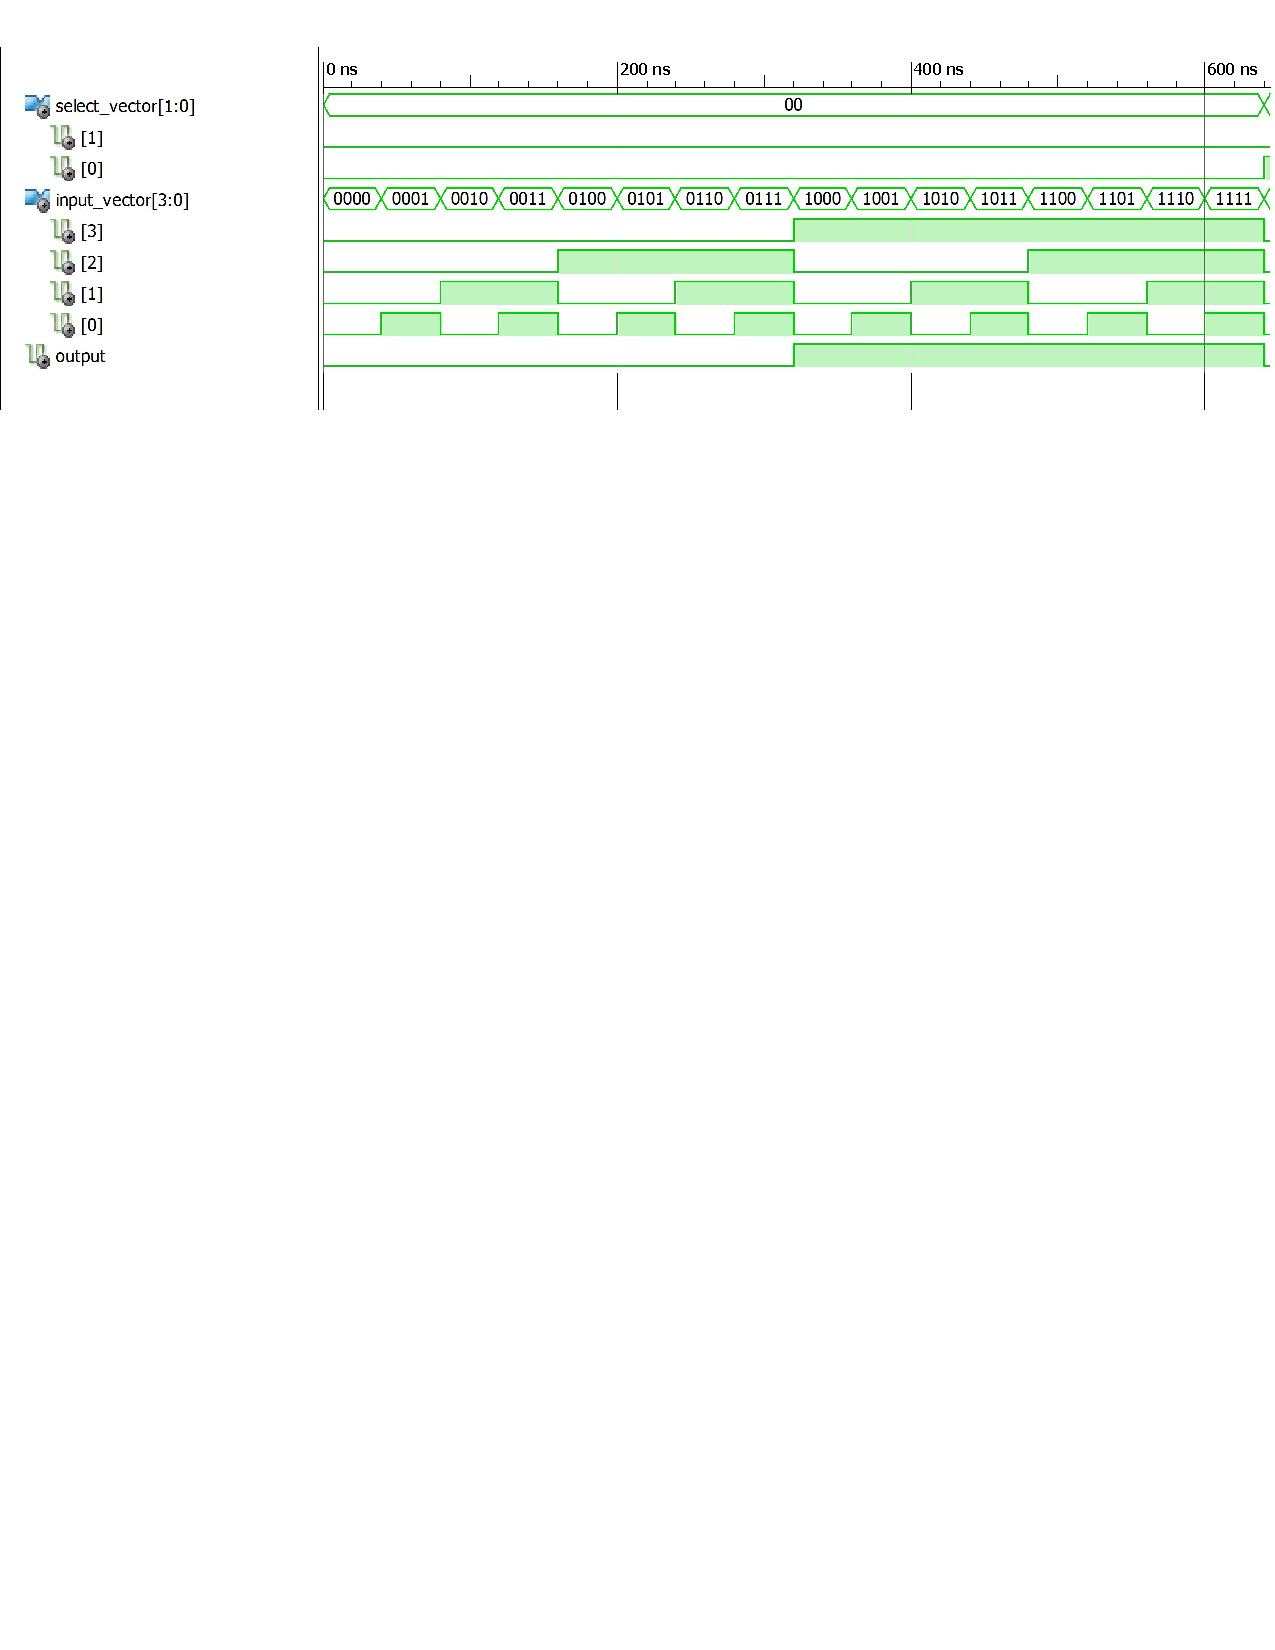
\includegraphics[scale=0.75,cframe=blue 0.5pt 3pt]{6aw-1.pdf}
    \caption{Simulation Waveform 0 ns to 700 ns  }
\end{figure}

\begin{figure}[H]
    \centering
    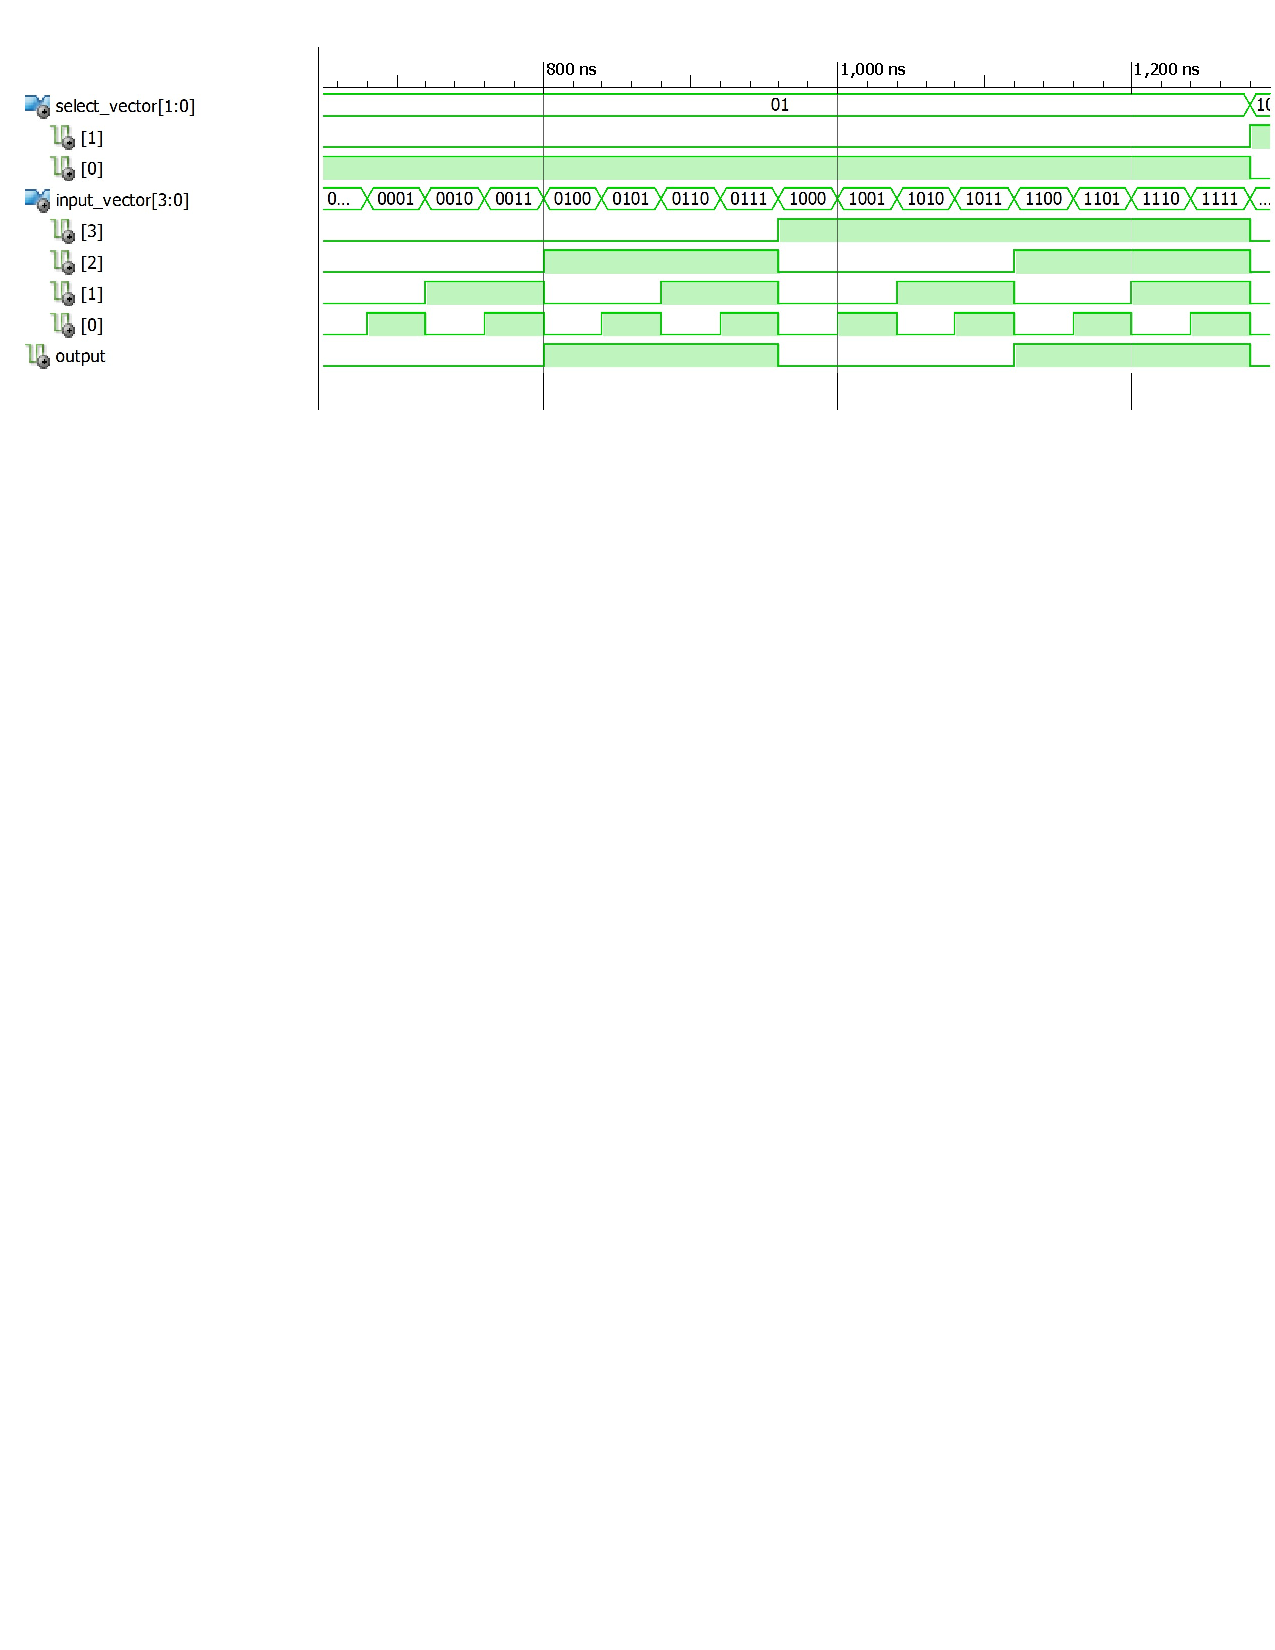
\includegraphics[scale=0.75,cframe=blue 0.5pt 3pt]{6aw-2.pdf}
    \caption{Simulation Waveform 700 ns to 1300 ns }
\end{figure}

\begin{figure}[H]
    \centering
    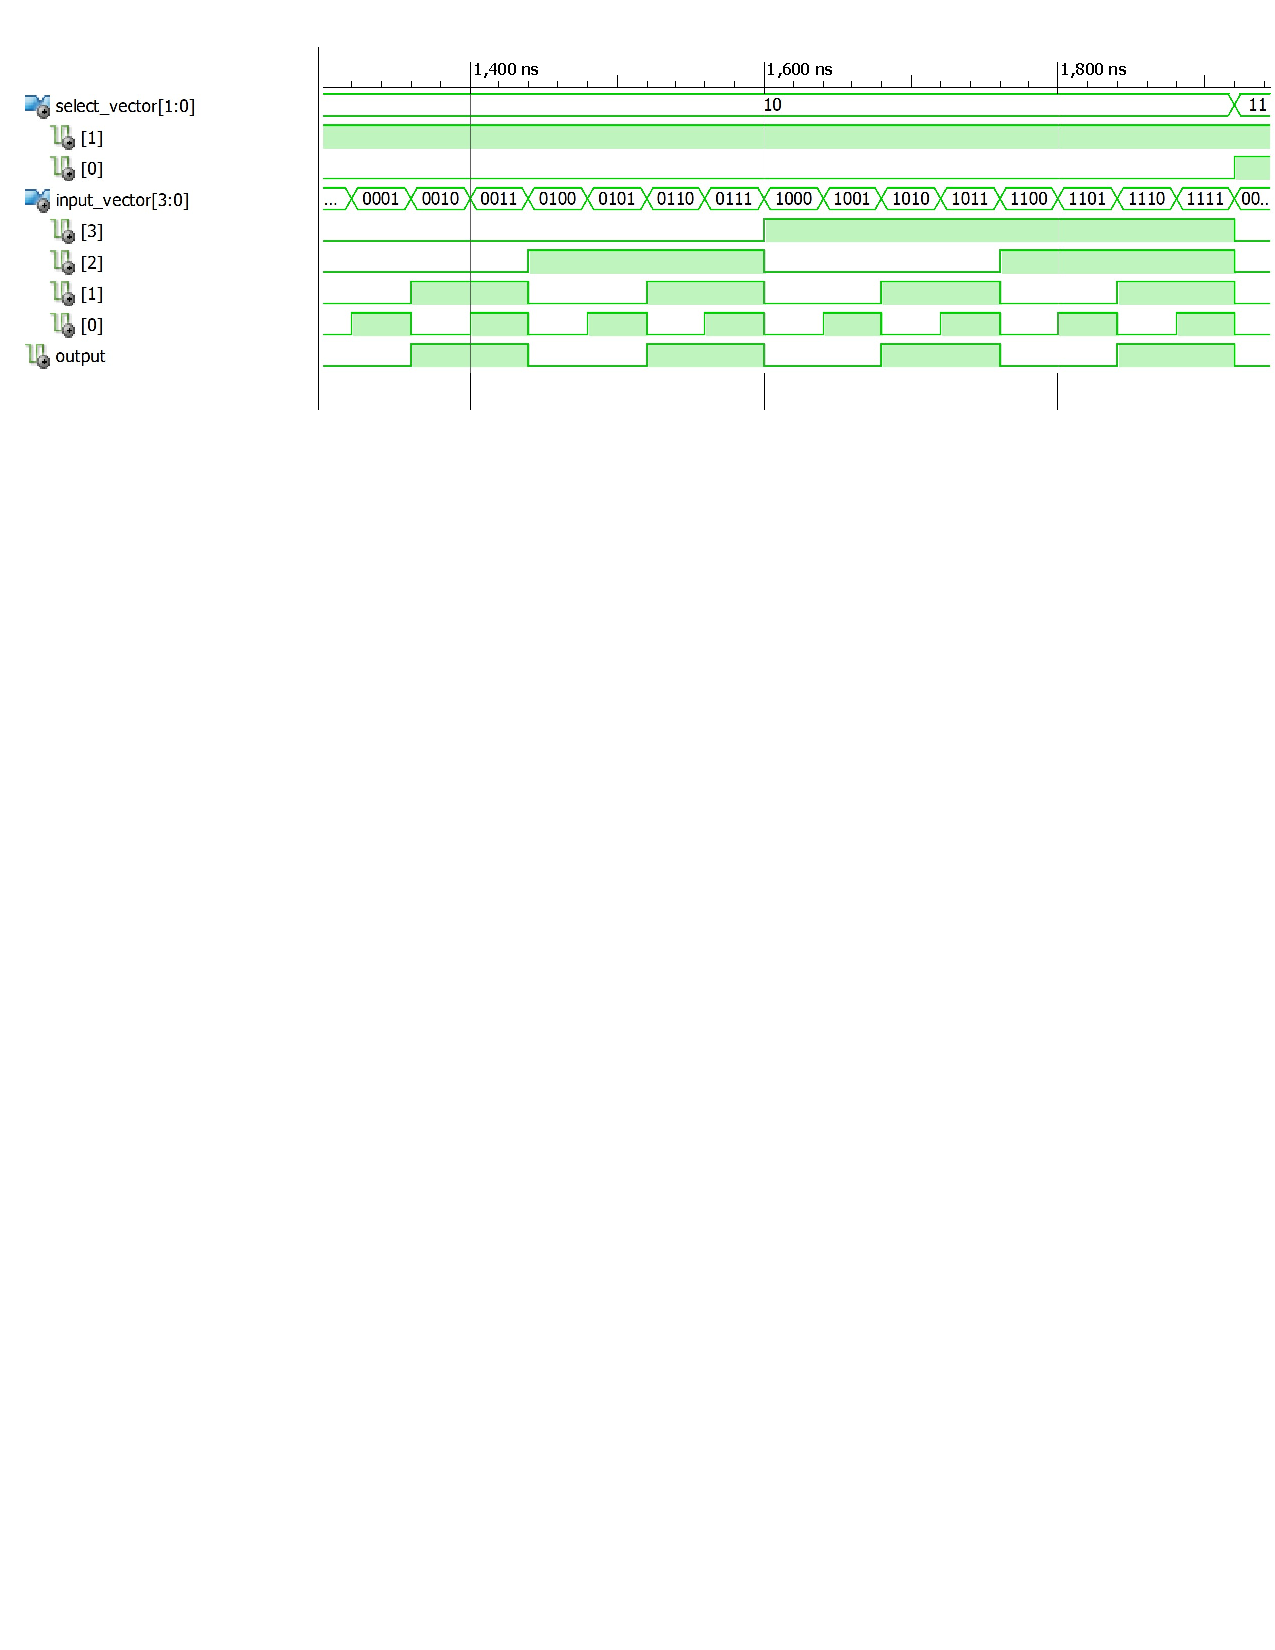
\includegraphics[scale=0.75,cframe=blue 0.5pt 3pt]{6aw-3.pdf}
    \caption{Simulation Waveform 1300 ns to 1900 ns  }
\end{figure}


\begin{figure}[H]
    \centering
    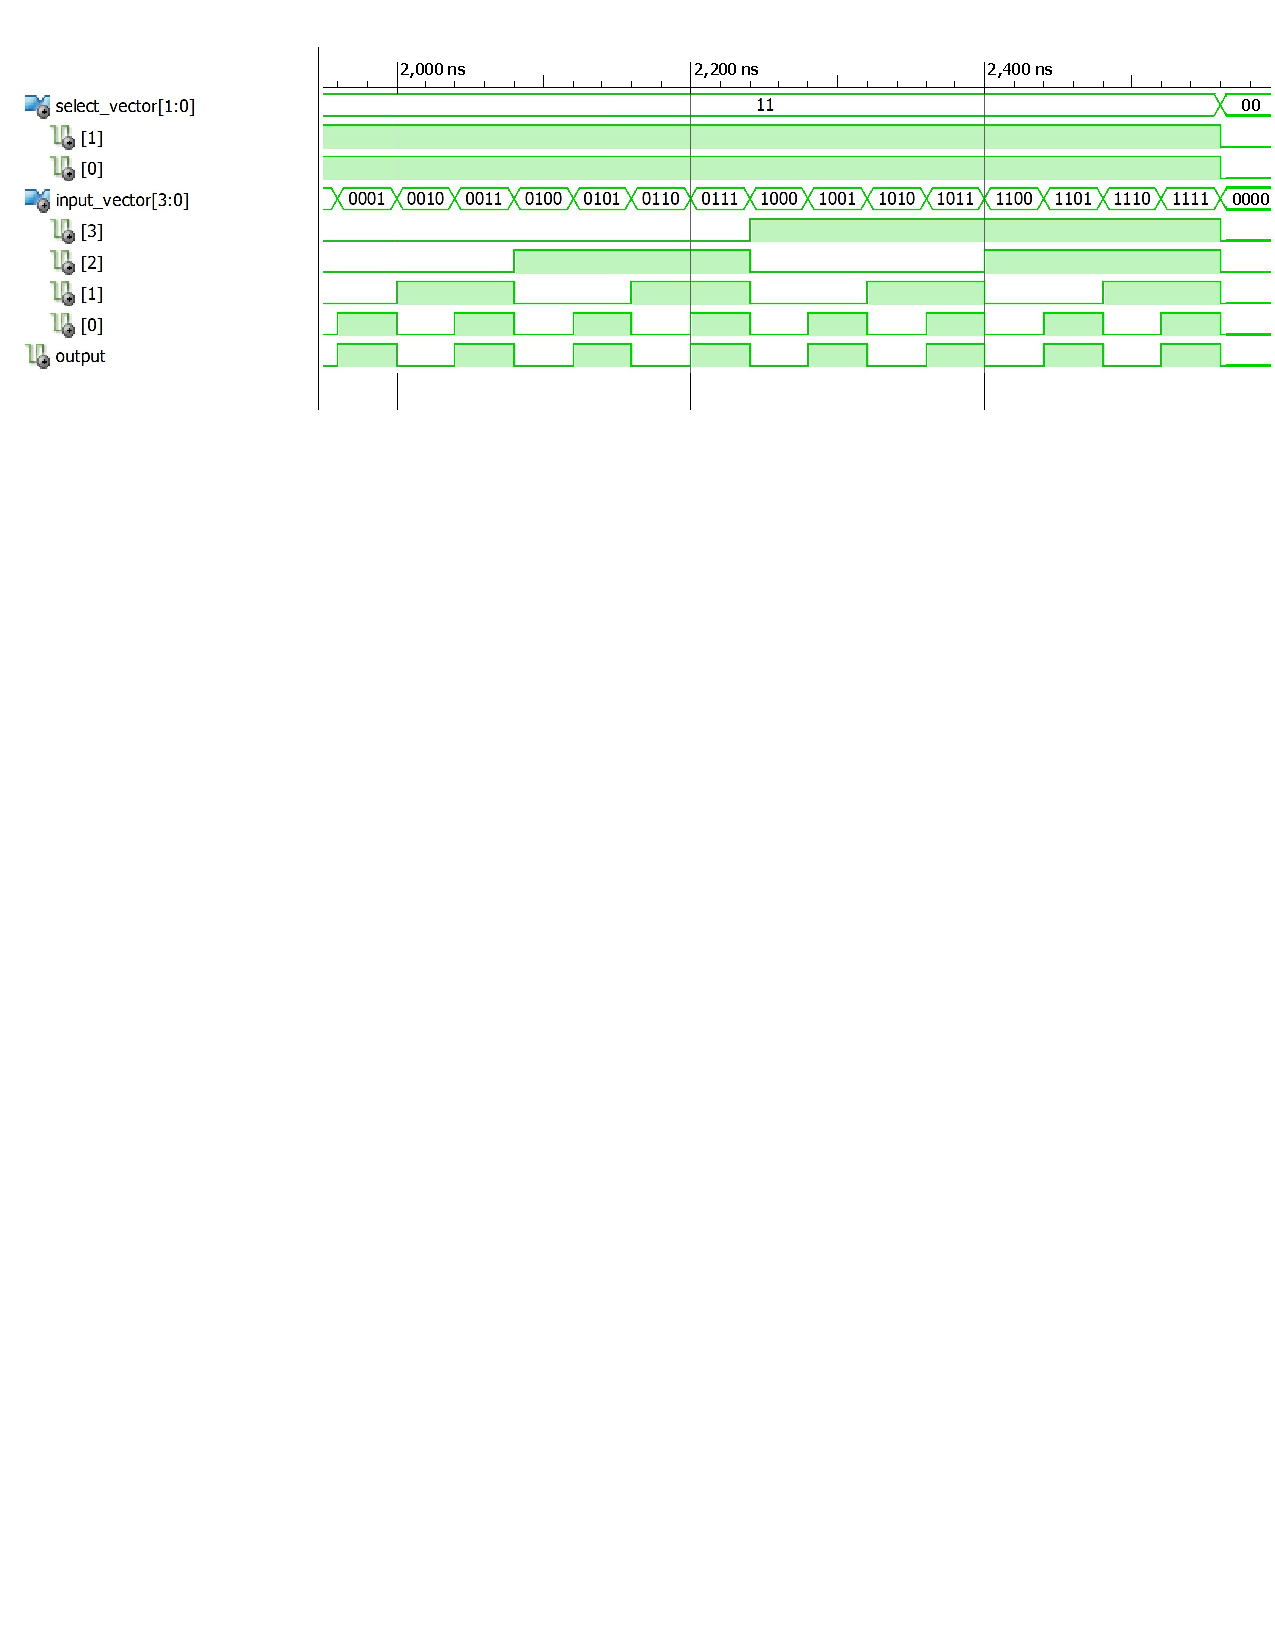
\includegraphics[scale=0.75,cframe=blue 0.5pt 3pt]{6aw-4.pdf}
    \caption{Simulation Waveform 1900 ns to 2600 ns }
\end{figure}


%%%RTL simulation
\begin{figure}[H]
    \centering
    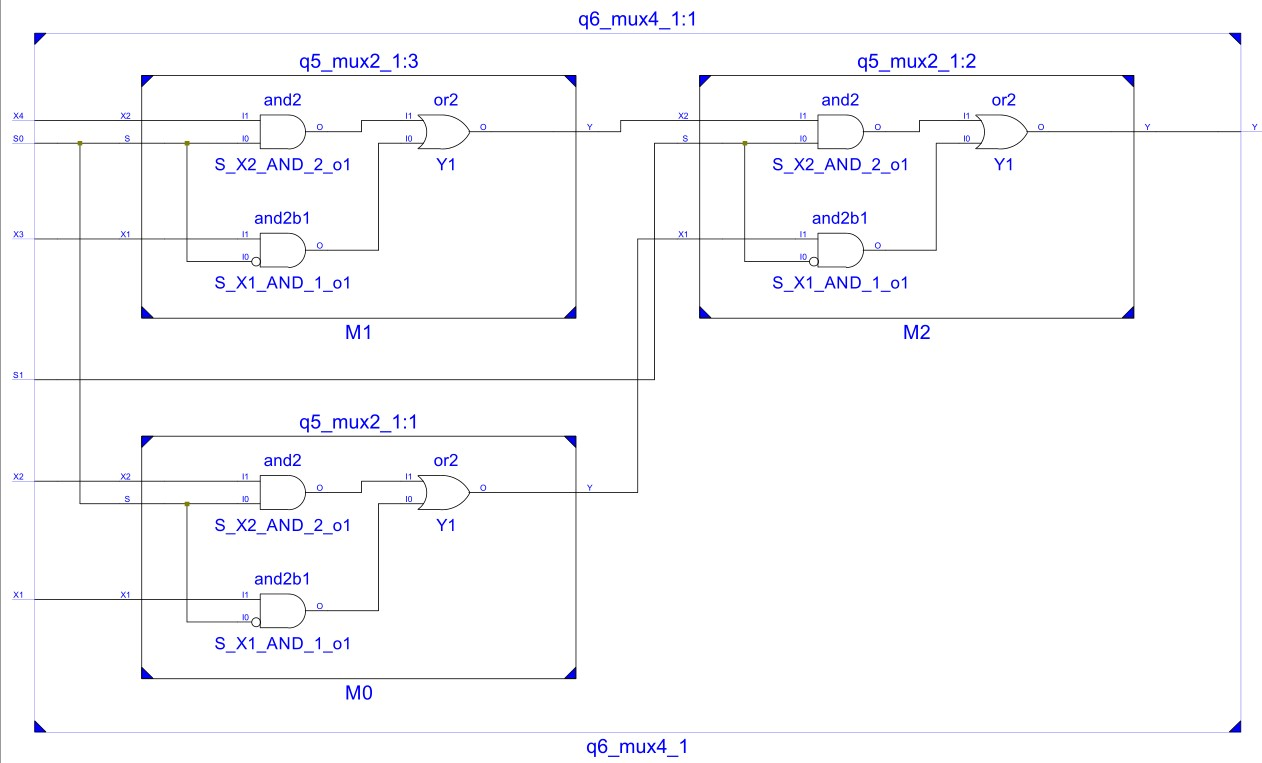
\includegraphics[scale=0.65,cframe=blue 0.5pt 3pt]{6s.jpg}
    \caption{RTL Schematic  }
\end{figure}



%%%%%%%%%%%%%
%%%%%%%%%%%%%%
%%%%%%%%%%%%%%
%%%%%%%%%%%%%%
%%%%%%%%%%%%%%
%%%%%%%%%%%%%%

%%%%%%%%%%%%%%%%%%%%%6666666666666666666666666666666666666

%%%%%%%%%%%%%%
%%%%%%%%%%%%%%
%%%%%%%%%%%%%%
%%%%%%%%%%%%%%
%%%%%%%%%%%%%%

\begin{Q}
    {
        Write VHDL code to implement a 4-bit adder/subtractor using four 1-bit full
        adders.
        \begin{enumerate}
            \item    Use a Structural architecture style with hierarchical design approach:
                  \begin{enumerate}
                      \item  Use 1-bit adder as the basic building block
                      \item Implement the 4-bit adder/subtractor using four 1-bit full adders.
                  \end{enumerate}
            \item  Write a VHDL test bench to verify the operation of the   4-bit adder/subtractor.
            \item Provide a simulation waveform depicting all possible input cases.
        \end{enumerate}
    }
\end{Q}

\addtocontents{lof}{\protect\subsection*{\HRule \\ Problem 7 \\ \HRule}}
\addtocontents{lol}{\protect\subsection*{\HRule \\ Problem 7 \\ \HRule}}

The required Boolean equation is :
\begin{align*}
    S=X \oplus Y \oplus  C_{in} \\
    C_{out}=XY + (X \oplus  Y) C_{in}
\end{align*}


\HRule
\anscode{ XOR gate implementation } {q7-xor.vhd}
\HRule

\HRule
\anscode{ Full adder implementation } {full-adder.vhd}
\HRule

\HRule
\anscode{ 4-bit adder/subtractor implementation using four 1-bit full-adder: Structural model } {q7-st.vhd}
\HRule


\HRule
\anscode{ Testbench for all possible cases } {q7-tb.vhd}
\HRule


\begin{figure}[H]
    \centering
    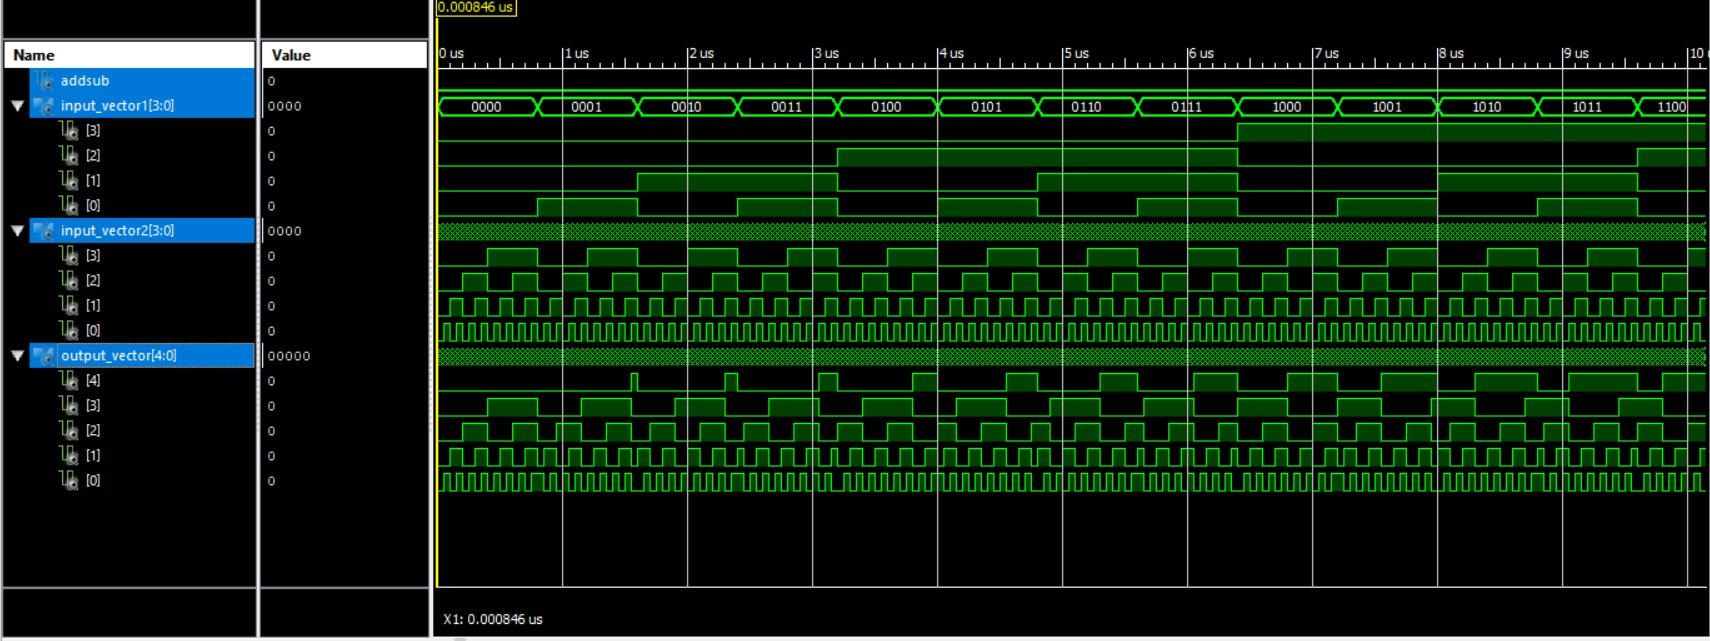
\includegraphics[scale=0.5,cframe=blue 0.5pt 3pt]{7aw.jpg}
    \caption{Simulation Waveform 4 bit Adder }
\end{figure}


\begin{figure}[H]
    \centering
    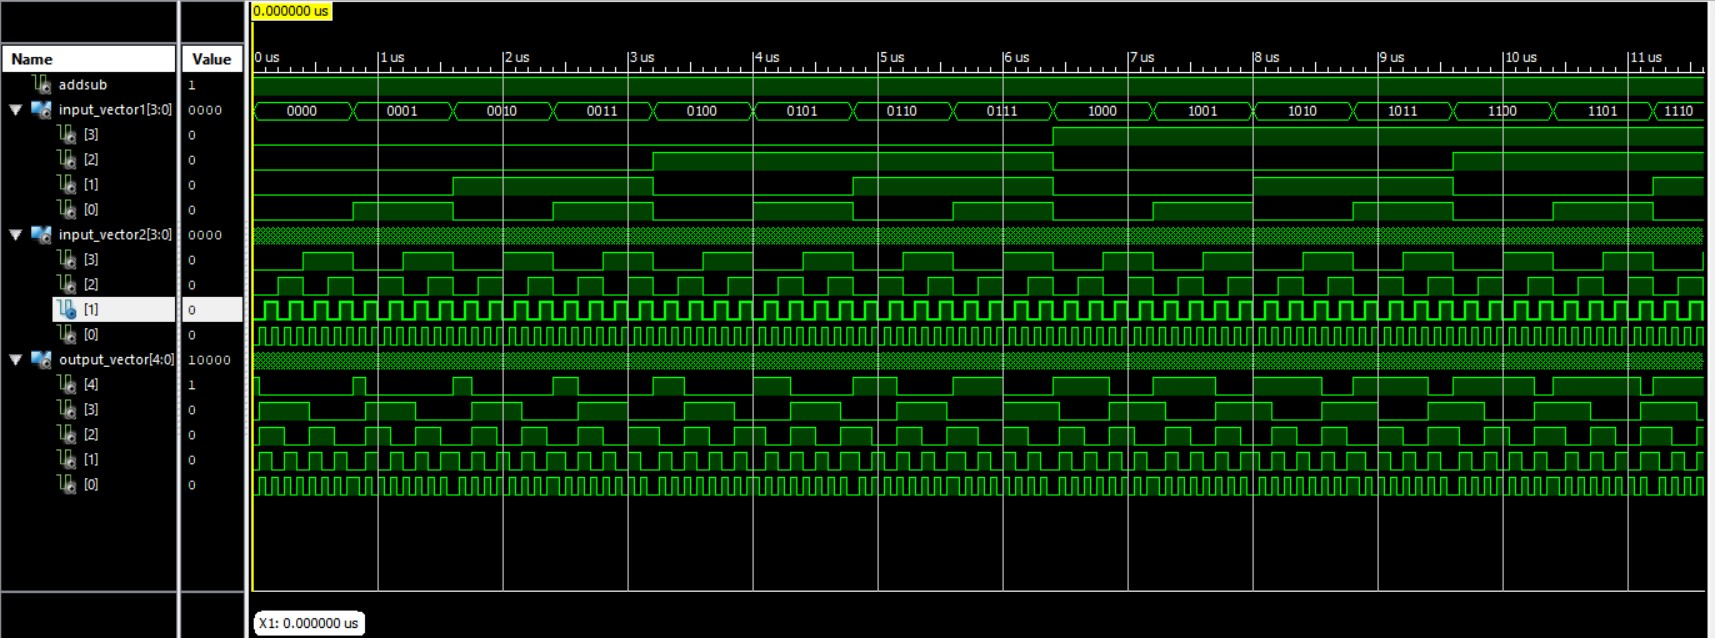
\includegraphics[scale=0.5,cframe=blue 0.5pt 3pt]{7sw.jpg}
    \caption{Simulation Waveform for 4 bit Subtractor }
\end{figure}

%%%RTL simulation
\begin{figure}[H]
    \centering
    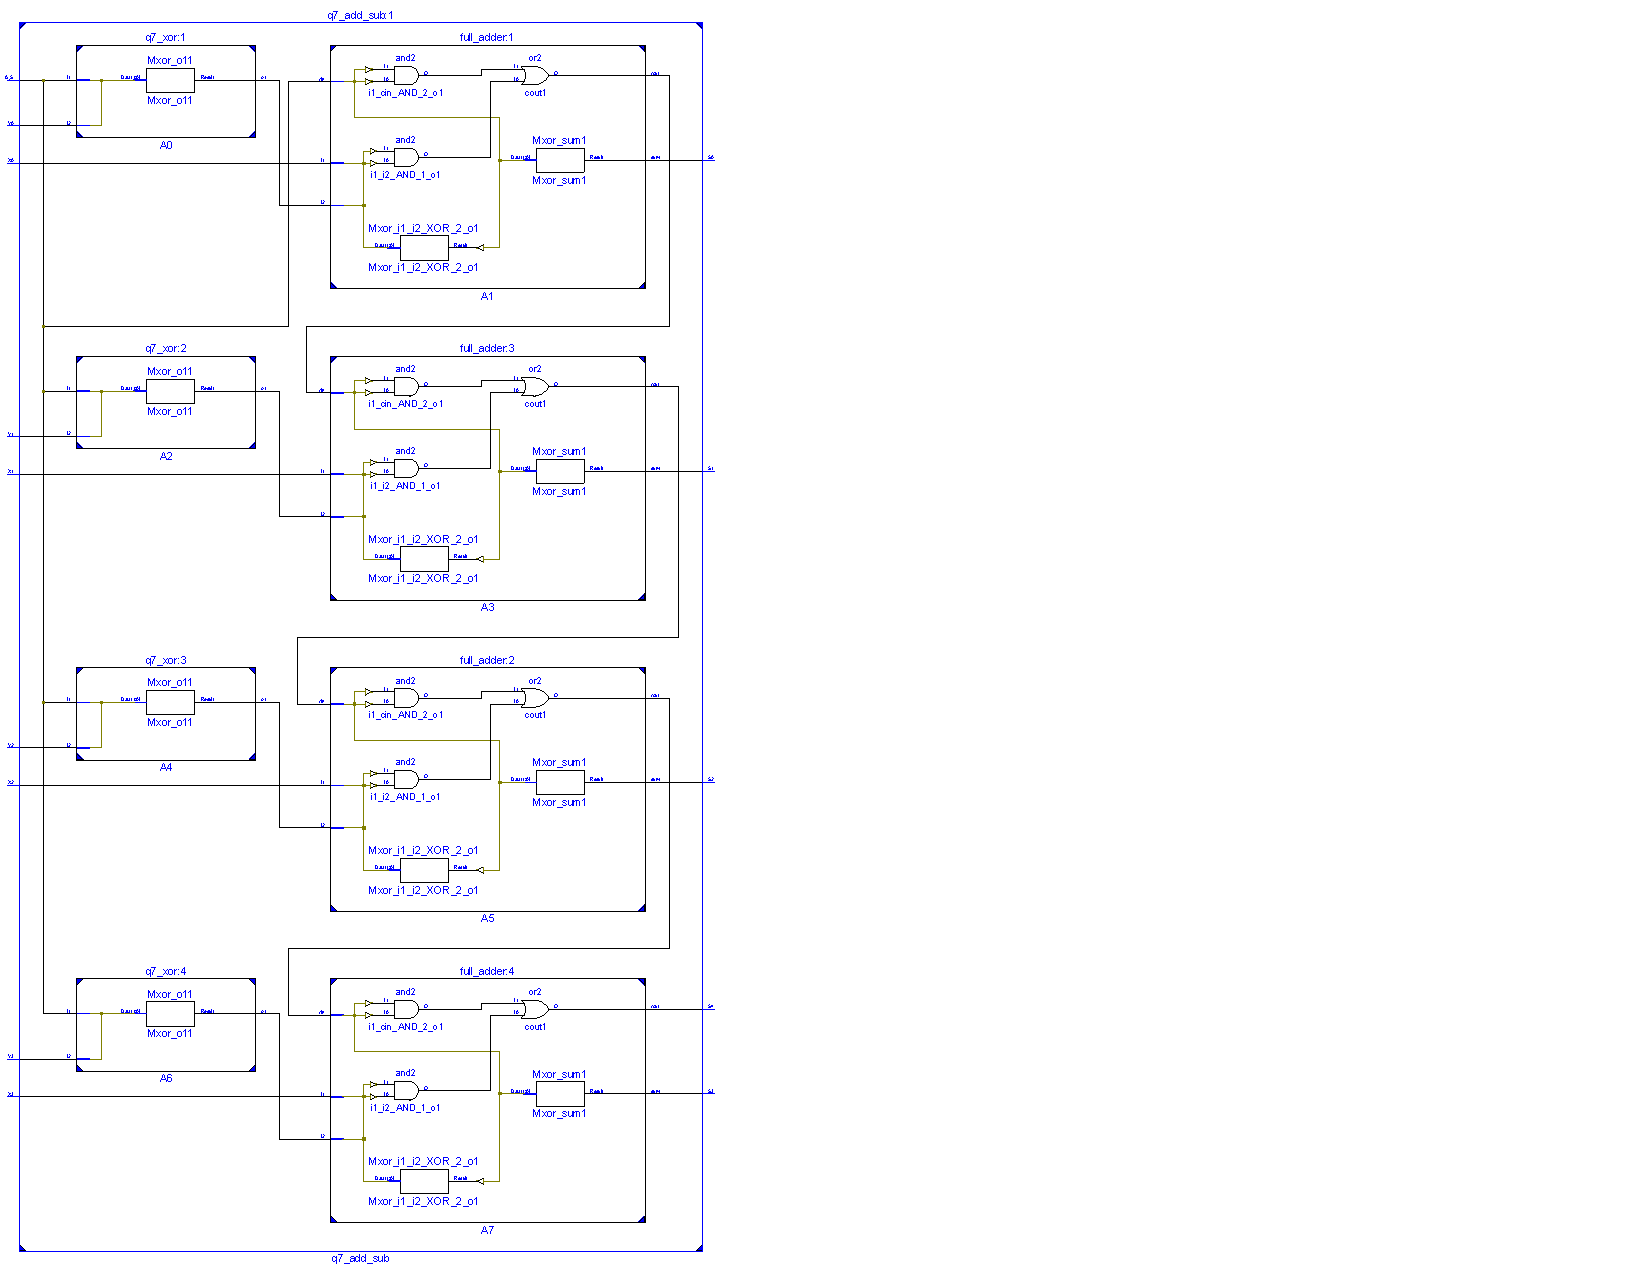
\includegraphics[scale=1.23,cframe=blue 0.5pt 3pt]{7s.pdf}
    \caption{RTL Schematic  }
\end{figure}




\section{Conclusion}

In this Lab we programs various circuits  in VHDL using Xilinx.We also familiarize ourselves with different architectural model like dataflow, behavioral and structural. Different waveforms and RTL schematic are included in this report.




\end{document}